\documentclass[10pt,xcolor=svgnames,aspectratio=169]{beamer} %Beamer
\usepackage{palatino} %font type
\usefonttheme{metropolis} %Type of slides
\usefonttheme[onlymath]{serif} %font type Mathematical expressions
\usetheme[titleformat frame=smallcaps]{metropolis} %This adds a bar at the beginning of each section.
% \usetheme[progressbar=frametitle,titleformat frame=smallcaps,numbering=counter]{metropolis}
% \useoutertheme[subsection=false]{miniframes} %Circles in the top of each frame, showing the slide of each section you are at

\usepackage{appendixnumberbeamer} %enumerate each slide without counting the appendix
% \setbeamercolor{progress bar}{fg=Maroon!70!Coral} %These are the colours of the progress bar. Notice that the names used are the svgnames
\setbeamercolor{title separator}{fg=DarkSalmon} %This is the line colour in the title slide
\setbeamercolor{structure}{fg=black} %Colour of the text of structure, numbers, items, blah. Not the big text.
\setbeamercolor{normal text}{fg=black!87} %Colour of normal text
\setbeamercolor{alerted text}{fg=DarkRed!60!Gainsboro} %Color of the alert box
\setbeamercolor{example text}{fg=Maroon!70!Coral} %Colour of the Example block text


\setbeamercolor{palette primary}{bg=NavyBlue!50!DarkOliveGreen, fg=white} %These are the colours of the background. Being this the main combination and so one. 
\setbeamercolor{palette secondary}{bg=NavyBlue!50!DarkOliveGreen, fg=white}
\setbeamercolor{palette tertiary}{bg=NavyBlue!40!Black, fg= white}
\setbeamercolor{section in toc}{fg=NavyBlue!40!Black} %Color of the text in the table of contents (toc)

\usepackage[utf8]{inputenc}
\usepackage[Symbol]{upgreek}
\usepackage{newtxmath}
\usepackage{multicol}
\usepackage[style=authortitle,backend=biber]{biblatex}
\addbibresource{bib.bib}
\usepackage[greek,english]{babel}
\usepackage{newunicodechar}
\usepackage{xcolor}
% \usepackage{polytable}


\newcommand{\themename}{\textbf{\textsc{bluetemp}\xspace}}%metropolis}}\xspace}

\newcommand{\awa}[2]{\mathrlap{#2}\phantom{#1}} % as wide as
\newcommand{\aha}[2]{\smash{\parbox{\linewidth}{#2}}\phantom{\parbox{\linewidth}{#1}}} % as high as
\newcommand{\parl}[1]{\parbox{\linewidth}{#1}} % as high as

\newcommand{\mi}[1]{\ensuremath{\mathit{#1}}}

\newunicodechar{→}{\ensuremath{\mathord{\rightarrow}}}
\newunicodechar{⇒}{\ensuremath{\mathord\Rightarrow}}
\newunicodechar{⊢}{\ensuremath{\mathord\vdash}}
\newunicodechar{⊨}{\ensuremath{\mathord\vDash}}
\newunicodechar{∀}{\ensuremath{\forall}}
\newunicodechar{ℕ}{\ensuremath{\mathbb{N}}}
\newunicodechar{ƛ}{\ensuremath{\lambdaslash}}
\newunicodechar{Γ}{\ensuremath{\varGamma}}
\newunicodechar{Δ}{\ensuremath{\varDelta}}
\newunicodechar{∋}{\ensuremath{\ni}}
\newunicodechar{μ}{\ensuremath{\mu}}
\newunicodechar{α}{\ensuremath{\alpha}}
\newunicodechar{ρ}{\ensuremath{\rho}}
\newunicodechar{σ}{\ensuremath{\sigma}}
\newunicodechar{τ}{\ensuremath{\tau}}
\newunicodechar{·}{\ensuremath{\mathord\cdotp}}
\newunicodechar{₁}{\ensuremath{_1}}
\newunicodechar{₂}{\ensuremath{_2}}
\newunicodechar{×}{\ensuremath{\times}}
\newunicodechar{ᵈ}{\ensuremath{^d}}
\newunicodechar{ω}{\ensuremath{\omega}}
\newunicodechar{λ}{\ensuremath{\lambda}}
\newunicodechar{▪}{\ensuremath{\blacksquare}}
\newunicodechar{‵}{\ensuremath{\mathord{^\backprime}}}
\newunicodechar{∷}{\ensuremath{::}}
\newunicodechar{∗}{\ensuremath{\mathord\ast}}
\newunicodechar{ℓ}{\ensuremath{\ell}}
\newunicodechar{∅}{\ensuremath{\emptyset}}


%% ODER: format ==         = "\mathrel{==}"
%% ODER: format /=         = "\neq "
%
%
\makeatletter
\@ifundefined{lhs2tex.lhs2tex.sty.read}%
  {\@namedef{lhs2tex.lhs2tex.sty.read}{}%
   \newcommand\SkipToFmtEnd{}%
   \newcommand\EndFmtInput{}%
   \long\def\SkipToFmtEnd#1\EndFmtInput{}%
  }\SkipToFmtEnd

\newcommand\ReadOnlyOnce[1]{\@ifundefined{#1}{\@namedef{#1}{}}\SkipToFmtEnd}
\usepackage{amstext}
\usepackage{amssymb}
\usepackage{stmaryrd}
\DeclareFontFamily{OT1}{cmtex}{}
\DeclareFontShape{OT1}{cmtex}{m}{n}
  {<5><6><7><8>cmtex8
   <9>cmtex9
   <10><10.95><12><14.4><17.28><20.74><24.88>cmtex10}{}
\DeclareFontShape{OT1}{cmtex}{m}{it}
  {<-> ssub * cmtt/m/it}{}
\newcommand{\texfamily}{\fontfamily{cmtex}\selectfont}
\DeclareFontShape{OT1}{cmtt}{bx}{n}
  {<5><6><7><8>cmtt8
   <9>cmbtt9
   <10><10.95><12><14.4><17.28><20.74><24.88>cmbtt10}{}
\DeclareFontShape{OT1}{cmtex}{bx}{n}
  {<-> ssub * cmtt/bx/n}{}
\newcommand{\tex}[1]{\text{\texfamily#1}}	% NEU

\newcommand{\Sp}{\hskip.33334em\relax}


\newcommand{\Conid}[1]{\mathit{#1}}
\newcommand{\Varid}[1]{\mathit{#1}}
\newcommand{\anonymous}{\kern0.06em \vbox{\hrule\@width.5em}}
\newcommand{\plus}{\mathbin{+\!\!\!+}}
\newcommand{\bind}{\mathbin{>\!\!\!>\mkern-6.7mu=}}
\newcommand{\rbind}{\mathbin{=\mkern-6.7mu<\!\!\!<}}% suggested by Neil Mitchell
\newcommand{\sequ}{\mathbin{>\!\!\!>}}
\renewcommand{\leq}{\leqslant}
\renewcommand{\geq}{\geqslant}
\usepackage{polytable}

%mathindent has to be defined
\@ifundefined{mathindent}%
  {\newdimen\mathindent\mathindent\leftmargini}%
  {}%

\def\resethooks{%
  \global\let\SaveRestoreHook\empty
  \global\let\ColumnHook\empty}
\newcommand*{\savecolumns}[1][default]%
  {\g@addto@macro\SaveRestoreHook{\savecolumns[#1]}}
\newcommand*{\restorecolumns}[1][default]%
  {\g@addto@macro\SaveRestoreHook{\restorecolumns[#1]}}
\newcommand*{\aligncolumn}[2]%
  {\g@addto@macro\ColumnHook{\column{#1}{#2}}}

\resethooks

\newcommand{\onelinecommentchars}{\quad-{}- }
\newcommand{\commentbeginchars}{\enskip\{-}
\newcommand{\commentendchars}{-\}\enskip}

\newcommand{\visiblecomments}{%
  \let\onelinecomment=\onelinecommentchars
  \let\commentbegin=\commentbeginchars
  \let\commentend=\commentendchars}

\newcommand{\invisiblecomments}{%
  \let\onelinecomment=\empty
  \let\commentbegin=\empty
  \let\commentend=\empty}

\visiblecomments

\newlength{\blanklineskip}
\setlength{\blanklineskip}{0.66084ex}

\newcommand{\hsindent}[1]{\quad}% default is fixed indentation
\let\hspre\empty
\let\hspost\empty
\newcommand{\NB}{\textbf{NB}}
\newcommand{\Todo}[1]{$\langle$\textbf{To do:}~#1$\rangle$}

\EndFmtInput
\makeatother
%
%
%
%
%
%
% This package provides two environments suitable to take the place
% of hscode, called "plainhscode" and "arrayhscode". 
%
% The plain environment surrounds each code block by vertical space,
% and it uses \abovedisplayskip and \belowdisplayskip to get spacing
% similar to formulas. Note that if these dimensions are changed,
% the spacing around displayed math formulas changes as well.
% All code is indented using \leftskip.
%
% Changed 19.08.2004 to reflect changes in colorcode. Should work with
% CodeGroup.sty.
%
\ReadOnlyOnce{polycode.fmt}%
\makeatletter

\newcommand{\hsnewpar}[1]%
  {{\parskip=0pt\parindent=0pt\par\vskip #1\noindent}}

% can be used, for instance, to redefine the code size, by setting the
% command to \small or something alike
\newcommand{\hscodestyle}{}

% The command \sethscode can be used to switch the code formatting
% behaviour by mapping the hscode environment in the subst directive
% to a new LaTeX environment.

\newcommand{\sethscode}[1]%
  {\expandafter\let\expandafter\hscode\csname #1\endcsname
   \expandafter\let\expandafter\endhscode\csname end#1\endcsname}

% "compatibility" mode restores the non-polycode.fmt layout.

\newenvironment{compathscode}%
  {\par\noindent
   \advance\leftskip\mathindent
   \hscodestyle
   \let\\=\@normalcr
   \let\hspre\(\let\hspost\)%
   \pboxed}%
  {\endpboxed\)%
   \par\noindent
   \ignorespacesafterend}

\newcommand{\compaths}{\sethscode{compathscode}}

% "plain" mode is the proposed default.
% It should now work with \centering.
% This required some changes. The old version
% is still available for reference as oldplainhscode.

\newenvironment{plainhscode}%
  {\hsnewpar\abovedisplayskip
   \advance\leftskip\mathindent
   \hscodestyle
   \let\hspre\(\let\hspost\)%
   \pboxed}%
  {\endpboxed%
   \hsnewpar\belowdisplayskip
   \ignorespacesafterend}

\newenvironment{oldplainhscode}%
  {\hsnewpar\abovedisplayskip
   \advance\leftskip\mathindent
   \hscodestyle
   \let\\=\@normalcr
   \(\pboxed}%
  {\endpboxed\)%
   \hsnewpar\belowdisplayskip
   \ignorespacesafterend}

% Here, we make plainhscode the default environment.

\newcommand{\plainhs}{\sethscode{plainhscode}}
\newcommand{\oldplainhs}{\sethscode{oldplainhscode}}
\plainhs

% The arrayhscode is like plain, but makes use of polytable's
% parray environment which disallows page breaks in code blocks.

\newenvironment{arrayhscode}%
  {\hsnewpar\abovedisplayskip
   \advance\leftskip\mathindent
   \hscodestyle
   \let\\=\@normalcr
   \(\parray}%
  {\endparray\)%
   \hsnewpar\belowdisplayskip
   \ignorespacesafterend}

\newcommand{\arrayhs}{\sethscode{arrayhscode}}

% The mathhscode environment also makes use of polytable's parray 
% environment. It is supposed to be used only inside math mode 
% (I used it to typeset the type rules in my thesis).

\newenvironment{mathhscode}%
  {\parray}{\endparray}

\newcommand{\mathhs}{\sethscode{mathhscode}}

% texths is similar to mathhs, but works in text mode.

\newenvironment{texthscode}%
  {\(\parray}{\endparray\)}

\newcommand{\texths}{\sethscode{texthscode}}

% The framed environment places code in a framed box.

\def\codeframewidth{\arrayrulewidth}
\RequirePackage{calc}

\newenvironment{framedhscode}%
  {\parskip=\abovedisplayskip\par\noindent
   \hscodestyle
   \arrayrulewidth=\codeframewidth
   \tabular{@{}|p{\linewidth-2\arraycolsep-2\arrayrulewidth-2pt}|@{}}%
   \hline\framedhslinecorrect\\{-1.5ex}%
   \let\endoflinesave=\\
   \let\\=\@normalcr
   \(\pboxed}%
  {\endpboxed\)%
   \framedhslinecorrect\endoflinesave{.5ex}\hline
   \endtabular
   \parskip=\belowdisplayskip\par\noindent
   \ignorespacesafterend}

\newcommand{\framedhslinecorrect}[2]%
  {#1[#2]}

\newcommand{\framedhs}{\sethscode{framedhscode}}

% The inlinehscode environment is an experimental environment
% that can be used to typeset displayed code inline.

\newenvironment{inlinehscode}%
  {\(\def\column##1##2{}%
   \let\>\undefined\let\<\undefined\let\\\undefined
   \newcommand\>[1][]{}\newcommand\<[1][]{}\newcommand\\[1][]{}%
   \def\fromto##1##2##3{##3}%
   \def\nextline{}}{\) }%

\newcommand{\inlinehs}{\sethscode{inlinehscode}}

% The joincode environment is a separate environment that
% can be used to surround and thereby connect multiple code
% blocks.

\newenvironment{joincode}%
  {\let\orighscode=\hscode
   \let\origendhscode=\endhscode
   \def\endhscode{\def\hscode{\endgroup\def\@currenvir{hscode}\\}\begingroup}
   %\let\SaveRestoreHook=\empty
   %\let\ColumnHook=\empty
   %\let\resethooks=\empty
   \orighscode\def\hscode{\endgroup\def\@currenvir{hscode}}}%
  {\origendhscode
   \global\let\hscode=\orighscode
   \global\let\endhscode=\origendhscode}%

\makeatother
\EndFmtInput
%

\title{Syntax-Generic Operations, Reflectively Reified}
\author[Name]{Tzu-Chi Lin and Josh Ko} %With inst, you can change the institution they belong
\subtitle{Extended Abstract}
\institute[uni]{Institute of Information Science \\ Academia Sinica, Taiwan}
\date{\today}

\begin{document}
{
	\setbeamercolor{background canvas}{bg=NavyBlue!50!DarkOliveGreen, fg=white}
	\setbeamercolor{normal text}{fg=white}
	\setbeamercovered{transparent}
	\maketitle
}%This is the colour of the first slide. bg= background and fg=foreground

\metroset{titleformat frame=smallcaps} %This changes the titles for small caps

\note{Hello everyone, my name is Tzu-Chi, I am a research assistant at Academia Sinica in Taiwan.
Today I will be talking about the joint work of my advisor's and mine, the title is "Syntax-generic Operations, Reflectively Reified". So firstly we will see what are syntax-generic operations, then I will elaborate on what Reflectively reified means.}

% \begin{frame}[fragile]{Outline}
% \setbeamertemplate{section in toc}[sections numbered] %This is numbering the sections
% \tableofcontents[hideallsubsections] %You can comment this line if you want to show the subsections in the table of contents
% \end{frame}

%\note{Firstly, I will introduce some backgrounds and our motivations, including the existing work we base on. In general, we apply the techniques we introduced in our another work, "Datatype-Generic Programming Meets Elaborator Reflection", which Josh will present on Tuesday. We apply the techniques in that work on a common problem for depentely typed programmers. I will show you a demo if we have time, and most importantly, we want to know your opinions on it. Is this a better approach? Will you want to use it? Hopefully we can get some feedbacks after this talk.}


\begin{frame}[fragile]{Typical Language in Language}
\emph{Intrinsic typing} is common for $\uplambda$-calculus with De Bruijn indices.
	% \aha{%
	% 	\begin{code}
	% data _⊢_ : Context → Type → Set where
  % ‵_     : Γ ∋ A → Γ ⊢ A
  % ƛ_     : Γ , A ⊢ B → Γ ⊢ A ⇒ B
  % _·_    : Γ ⊢ A ⇒ B → Γ ⊢ A → Γ ⊢ B
  % ‵zero  : Γ ⊢ ‵ℕ
  % ‵suc_  : Γ ⊢ ‵ℕ → Γ ⊢ ‵ℕ
  % case   : Γ ⊢ ‵ℕ → Γ ⊢ A → Γ , ‵ℕ ⊢ A → Γ ⊢ A
  % μ_     : Γ , A ⊢ A → Γ ⊢ A
	% 	\end{code}
	% }{%
		\begin{columns}[T]
			\begin{column}{0.6\textwidth}
				\begin{hscode}\SaveRestoreHook
\column{B}{@{}>{\hspre}l<{\hspost}@{}}%
\column{3}{@{}>{\hspre}l<{\hspost}@{}}%
\column{10}{@{}>{\hspre}l<{\hspost}@{}}%
\column{E}{@{}>{\hspre}l<{\hspost}@{}}%
\>[B]{}\mathbf{data}\;\Varid{\char95 ⊢\char95 }\;\mathbin{:}\;\Conid{Context}\;\Varid{→}\;\Conid{Ty}\;\Varid{→}\;\Conid{Set}\;\mathbf{where}{}\<[E]%
\\
\>[B]{}\hsindent{3}{}\<[3]%
\>[3]{}\Varid{‵\char95 }\;{}\<[10]%
\>[10]{}\mathbin{:}\;\Conid{Γ}\;\Varid{∋}\;\Conid{A}\;\Varid{→}\;\Conid{Γ}\;\Varid{⊢}\;\Conid{A}{}\<[E]%
\\
\>[B]{}\hsindent{3}{}\<[3]%
\>[3]{}\Varid{ƛ\char95 }\;{}\<[10]%
\>[10]{}\mathbin{:}\;\Conid{Γ}\;\Varid{,}\;\Conid{A}\;\Varid{⊢}\;\Conid{B}\;\Varid{→}\;\Conid{Γ}\;\Varid{⊢}\;\Conid{A}\;\Varid{⇒}\;\Conid{B}{}\<[E]%
\\
\>[B]{}\hsindent{3}{}\<[3]%
\>[3]{}\Varid{\char95 ·\char95 }\;{}\<[10]%
\>[10]{}\mathbin{:}\;\Conid{Γ}\;\Varid{⊢}\;\Conid{A}\;\Varid{⇒}\;\Conid{B}\;\Varid{→}\;\Conid{Γ}\;\Varid{⊢}\;\Conid{A}\;\Varid{→}\;\Conid{Γ}\;\Varid{⊢}\;\Conid{B}{}\<[E]%
\ColumnHook
\end{hscode}\resethooks
			\end{column}
			\begin{column}{0.6\textwidth}
				\begin{hscode}\SaveRestoreHook
\column{B}{@{}>{\hspre}l<{\hspost}@{}}%
\column{3}{@{}>{\hspre}l<{\hspost}@{}}%
\column{8}{@{}>{\hspre}l<{\hspost}@{}}%
\column{E}{@{}>{\hspre}l<{\hspost}@{}}%
\>[B]{}\mathbf{data}\;\Conid{Ty}\;\mathbin{:}\;\Conid{Set}\;\mathbf{where}{}\<[E]%
\\
\>[B]{}\hsindent{3}{}\<[3]%
\>[3]{}\Varid{α}\;{}\<[8]%
\>[8]{}\mathbin{:}\;\Conid{Ty}{}\<[E]%
\\
\>[B]{}\hsindent{3}{}\<[3]%
\>[3]{}\Varid{\char95 ⇒\char95 }\;{}\<[8]%
\>[8]{}\mathbin{:}\;\Conid{Ty}\;\Varid{→}\;\Conid{Ty}\;\Varid{→}\;\Conid{Ty}{}\<[E]%
\\[\blanklineskip]%
\>[B]{}\mathbf{data}\;\Conid{Context}\;(\Conid{A}\;\mathbin{:}\;\Conid{Set})\;\mathbin{:}\;\Conid{Set}\;\mathbf{where}{}\<[E]%
\\
\>[B]{}\hsindent{3}{}\<[3]%
\>[3]{}\Varid{∅}\;{}\<[8]%
\>[8]{}\mathbin{:}\;\Conid{Context}\;\Conid{A}{}\<[E]%
\\
\>[B]{}\hsindent{3}{}\<[3]%
\>[3]{}\Varid{\char95 ,\char95 }\;{}\<[8]%
\>[8]{}\mathbin{:}\;(\Conid{Γ}\;\mathbin{:}\;\Conid{Context}\;\Conid{A})\;\Varid{→}\;\Conid{A}\;\Varid{→}\;\Conid{Context}\;\Conid{A}{}\<[E]%
\\[\blanklineskip]%
\>[B]{}\mathbf{data}\;\Varid{\char95 ∋\char95 }\;\mathbin{:}\;\Conid{Context}\;\Varid{→}\;\Conid{Ty}\;\Varid{→}\;\Conid{Set}\;\mathbf{where}{}\<[E]%
\\
\>[B]{}\hsindent{3}{}\<[3]%
\>[3]{}\Varid{z}\;\mathbin{:}\;\Conid{Γ}\;\Varid{,}\;\Conid{A}\;\Varid{∋}\;\Conid{A}{}\<[E]%
\\
\>[B]{}\hsindent{3}{}\<[3]%
\>[3]{}\Varid{s}\;\mathbin{:}\;\Conid{Γ}\;\Varid{∋}\;\Conid{A}\;\Varid{→}\;\Conid{Γ}\;\Varid{,}\;\Conid{B}\;\Varid{∋}\;\Conid{A}{}\<[E]%
\ColumnHook
\end{hscode}\resethooks
			\end{column}
		\end{columns}
	% }
\end{frame}

\note{For starters, Let's take a look at a common thing dependently typed programmers would do, that is defining a programming language in a dependently typed programming language, such as Agda. Here is an example of the syntax of a language defined in Agda. It's a simply-typed lambda calculus. We define a datatype called Ty to describe the possible types for this language, a term has either a single type or a function type. Here \mi{Context} is defined as the List of Ty. And we have a simple ``has'' relation that represents variables. For if a variable is typed it must be in the context. And we know that a simply typed lambda calculus has three constructions, each corresponding a a typing rule. Here are three constructors, each of them corresponds to the variable rule, the abstraction rule, and the application rule. We can see for a term to be constructed, it must be well-typed by definition, that's what we call intrinsic typing.}

\begin{frame}{Scope-safe Operations}
	\begin{hscode}\SaveRestoreHook
\column{B}{@{}>{\hspre}l<{\hspost}@{}}%
\column{19}{@{}>{\hspre}l<{\hspost}@{}}%
\column{22}{@{}>{\hspre}l<{\hspost}@{}}%
\column{35}{@{}>{\hspre}l<{\hspost}@{}}%
\column{44}{@{}>{\hspre}l<{\hspost}@{}}%
\column{E}{@{}>{\hspre}l<{\hspost}@{}}%
\>[B]{}\Varid{rename}\;\mathbin{:}\;\Varid{∀}\;\{\mskip1.5mu \Conid{Γ}\;\Conid{Δ}\mskip1.5mu\}\;{}\<[19]%
\>[19]{}\Varid{→}\;(\Varid{∀}\;\{\mskip1.5mu \Conid{A}\mskip1.5mu\}\;\Varid{→}\;\Conid{Γ}\;\Varid{∋}\;{}\<[35]%
\>[35]{}\Conid{A}\;\Varid{→}\;\Conid{Δ}\;\Varid{∋}\;{}\<[44]%
\>[44]{}\Conid{A})\;{}\<[E]%
\\
\>[19]{}\Varid{→}\;(\Varid{∀}\;\{\mskip1.5mu \Conid{A}\mskip1.5mu\}\;\Varid{→}\;\Conid{Γ}\;\Varid{⊢}\;{}\<[35]%
\>[35]{}\Conid{A}\;\Varid{→}\;\Conid{Δ}\;\Varid{⊢}\;{}\<[44]%
\>[44]{}\Conid{A}){}\<[E]%
\\
\>[B]{}\Varid{rename}\;\Varid{ρ}\;(\Varid{‵}\;\Varid{x})\;{}\<[19]%
\>[19]{}\mathrel{=}\;{}\<[22]%
\>[22]{}\Varid{‵}\;(\Varid{ρ}\;\Varid{x}){}\<[E]%
\\
\>[B]{}\Varid{rename}\;\Varid{ρ}\;(\Varid{ƛ}\;\Conid{N})\;{}\<[19]%
\>[19]{}\mathrel{=}\;{}\<[22]%
\>[22]{}\Varid{ƛ}\;(\Varid{rename}\;(\Varid{ext}\;\Varid{ρ})\;\Conid{N}){}\<[E]%
\\
\>[B]{}\Varid{rename}\;\Varid{ρ}\;(\Conid{L}\;\Varid{·}\;\Conid{M})\;{}\<[19]%
\>[19]{}\mathrel{=}\;{}\<[22]%
\>[22]{}(\Varid{rename}\;\Varid{ρ}\;\Conid{L})\;\Varid{·}\;(\Varid{rename}\;\Varid{ρ}\;\Conid{M}){}\<[E]%
\ColumnHook
\end{hscode}\resethooks
\end{frame}

\note{Then let's define some operations on this syntax. Again, because of intrinsic typing, such operations are scope-safe. For example, a \mi{rename} function says that if there's a mapping from every variable in a context $\varGamma$ to the other context $\varDelta$, we can always find a mapping from every term that is typed in $\varGamma$ to a term typed in $\varDelta$. Because we can remap every variable in that term. If we encounter a subterm that has a extended context, for example, the case of lambda abstraction, the variable mapping should be extended accordingly. We can see that rename is still called recursively, but the variable mapping function is modified with ext.}

\begin{frame}[fragile]{Repetition}
\emph{Intrinsic typing} is common for $\uplambda$-calculus with De Bruijn indices.
	\parl{
	\begin{hscode}\SaveRestoreHook
\column{B}{@{}>{\hspre}l<{\hspost}@{}}%
\column{3}{@{}>{\hspre}l<{\hspost}@{}}%
\column{10}{@{}>{\hspre}l<{\hspost}@{}}%
\column{E}{@{}>{\hspre}l<{\hspost}@{}}%
\>[B]{}\mathbf{data}\;\Conid{Ty}\;\mathbin{:}\;\Conid{Set}\;\mathbf{where}{}\<[E]%
\\
\>[B]{}\hsindent{3}{}\<[3]%
\>[3]{}\Varid{...}{}\<[E]%
\\
\>[B]{}\hsindent{3}{}\<[3]%
\>[3]{}\Varid{‵ℕ}\;\mathbin{:}\;\Conid{Ty}{}\<[E]%
\\[\blanklineskip]%
\>[B]{}\mathbf{data}\;\Varid{\char95 ⊢\char95 }\;\mathbin{:}\;\Conid{Context}\;\Varid{→}\;\Conid{Ty}\;\Varid{→}\;\Conid{Set}\;\mathbf{where}{}\<[E]%
\\
\>[B]{}\hsindent{3}{}\<[3]%
\>[3]{}\Varid{...}{}\<[E]%
\\
\>[B]{}\hsindent{3}{}\<[3]%
\>[3]{}\Varid{‵zero}\;{}\<[10]%
\>[10]{}\mathbin{:}\;\Conid{Γ}\;\Varid{⊢}\;\Varid{‵ℕ}{}\<[E]%
\\
\>[B]{}\hsindent{3}{}\<[3]%
\>[3]{}\Varid{‵suc\char95 }\;{}\<[10]%
\>[10]{}\mathbin{:}\;\Conid{Γ}\;\Varid{⊢}\;\Varid{‵ℕ}\;\Varid{→}\;\Conid{Γ}\;\Varid{⊢}\;\Varid{‵ℕ}{}\<[E]%
\\
\>[B]{}\hsindent{3}{}\<[3]%
\>[3]{}\Varid{case}\;{}\<[10]%
\>[10]{}\mathbin{:}\;\Conid{Γ}\;\Varid{⊢}\;\Varid{‵ℕ}\;\Varid{→}\;\Conid{Γ}\;\Varid{⊢}\;\Conid{A}\;\Varid{→}\;\Conid{Γ}\;\Varid{,}\;\Varid{‵ℕ}\;\Varid{⊢}\;\Conid{A}\;\Varid{→}\;\Conid{Γ}\;\Varid{⊢}\;\Conid{A}{}\<[E]%
\\
\>[B]{}\hsindent{3}{}\<[3]%
\>[3]{}\Varid{μ\char95 }\;{}\<[10]%
\>[10]{}\mathbin{:}\;\Conid{Γ}\;\Varid{,}\;\Conid{A}\;\Varid{⊢}\;\Conid{A}\;\Varid{→}\;\Conid{Γ}\;\Varid{⊢}\;\Conid{A}{}\<[E]%
\ColumnHook
\end{hscode}\resethooks
	}
\end{frame}

\note{Now what if we extend the language? we might want natural number primitives in our language, so we extend the Ty datatype with a new type, we add four typing rules, two of them, zero and suc are for constructing natural numbers, and another two rules are for branching and recursion.}

\begin{frame}[fragile]{Repetition}
		\begin{hscode}\SaveRestoreHook
\column{B}{@{}>{\hspre}l<{\hspost}@{}}%
\column{19}{@{}>{\hspre}l<{\hspost}@{}}%
\column{25}{@{}>{\hspre}l<{\hspost}@{}}%
\column{28}{@{}>{\hspre}l<{\hspost}@{}}%
\column{34}{@{}>{\hspre}l<{\hspost}@{}}%
\column{35}{@{}>{\hspre}l<{\hspost}@{}}%
\column{44}{@{}>{\hspre}l<{\hspost}@{}}%
\column{E}{@{}>{\hspre}l<{\hspost}@{}}%
\>[B]{}\Varid{rename}\;\mathbin{:}\;\Varid{∀}\;\{\mskip1.5mu \Conid{Γ}\;\Conid{Δ}\mskip1.5mu\}\;{}\<[19]%
\>[19]{}\Varid{→}\;(\Varid{∀}\;\{\mskip1.5mu \Conid{A}\mskip1.5mu\}\;\Varid{→}\;\Conid{Γ}\;\Varid{∋}\;{}\<[35]%
\>[35]{}\Conid{A}\;\Varid{→}\;\Conid{Δ}\;\Varid{∋}\;{}\<[44]%
\>[44]{}\Conid{A})\;{}\<[E]%
\\
\>[19]{}\Varid{→}\;(\Varid{∀}\;\{\mskip1.5mu \Conid{A}\mskip1.5mu\}\;\Varid{→}\;\Conid{Γ}\;\Varid{⊢}\;{}\<[35]%
\>[35]{}\Conid{A}\;\Varid{→}\;\Conid{Δ}\;\Varid{⊢}\;{}\<[44]%
\>[44]{}\Conid{A}){}\<[E]%
\\
\>[B]{}\Varid{...}{}\<[E]%
\\
\>[B]{}\Varid{rename}\;\Varid{ρ}\;(\Varid{‵zero})\;{}\<[25]%
\>[25]{}\mathrel{=}\;{}\<[28]%
\>[28]{}\Varid{‵zero}{}\<[E]%
\\
\>[B]{}\Varid{rename}\;\Varid{ρ}\;(\Varid{‵suc}\;\Conid{M})\;{}\<[25]%
\>[25]{}\mathrel{=}\;{}\<[28]%
\>[28]{}\Varid{‵suc}\;(\Varid{rename}\;\Varid{ρ}\;\Conid{M}){}\<[E]%
\\
\>[B]{}\Varid{rename}\;\Varid{ρ}\;(\Varid{case}\;\Conid{L}\;\Conid{M}\;\Conid{N})\;{}\<[25]%
\>[25]{}\mathrel{=}\;{}\<[28]%
\>[28]{}\Varid{case}\;{}\<[34]%
\>[34]{}(\Varid{rename}\;\Varid{ρ}\;\Conid{L})\;{}\<[E]%
\\
\>[34]{}(\Varid{rename}\;\Varid{ρ}\;\Conid{M})\;{}\<[E]%
\\
\>[34]{}(\Varid{rename}\;(\Varid{ext}\;\Varid{ρ})\;\Conid{N}){}\<[E]%
\\
\>[B]{}\Varid{rename}\;\Varid{ρ}\;(\Varid{μ}\;\Conid{N})\;{}\<[25]%
\>[25]{}\mathrel{=}\;{}\<[28]%
\>[28]{}\Varid{μ}\;(\Varid{rename}\;(\Varid{ext}\;\Varid{ρ})\;\Conid{N}){}\<[E]%
\ColumnHook
\end{hscode}\resethooks
\end{frame}

\note{If we want a rename function for this extended language, we can copy and paste the rename we just defined and add a new clause for each constructor. The patterns still follow, a renaming always take a term from a constructor to one with the same constructor, if encounter subterm, call rename recursively, if there's context extension, extend the variable mapping as well. So no matter how many constructors there are we follow the same logic.}

\begin{frame}[fragile]{Repetition}
Change/extend the object language even further:
		\begin{hscode}\SaveRestoreHook
\column{B}{@{}>{\hspre}l<{\hspost}@{}}%
\column{3}{@{}>{\hspre}l<{\hspost}@{}}%
\column{9}{@{}>{\hspre}l<{\hspost}@{}}%
\column{13}{@{}>{\hspre}l<{\hspost}@{}}%
\column{E}{@{}>{\hspre}l<{\hspost}@{}}%
\>[B]{}\mathbf{data}\;\Varid{\char95 ⊢\char95 }\;\mathbin{:}\;\Conid{Context}\;\Varid{→}\;\Conid{Ty}\;\Varid{→}\;\Conid{Set}\;\mathbf{where}{}\<[E]%
\\
\>[B]{}\hsindent{9}{}\<[9]%
\>[9]{}\Varid{...}{}\<[E]%
\\
\>[B]{}\hsindent{3}{}\<[3]%
\>[3]{}\Varid{con}\;{}\<[13]%
\>[13]{}\mathbin{:}\;\Conid{ℕ}\;\Varid{→}\;\Conid{Γ}\;\Varid{⊢}\;\Conid{Nat}{}\<[E]%
\\
\>[B]{}\hsindent{3}{}\<[3]%
\>[3]{}\Varid{\char95 ‵∗\char95 }\;{}\<[13]%
\>[13]{}\mathbin{:}\;\Conid{Γ}\;\Varid{⊢}\;\Conid{Nat}\;\Varid{→}\;\Conid{Γ}\;\Varid{⊢}\;\Conid{Nat}\;\Varid{→}\;\Conid{Γ}\;\Varid{⊢}\;\Conid{Nat}{}\<[E]%
\\
\>[B]{}\hsindent{3}{}\<[3]%
\>[3]{}\Varid{‵let}\;{}\<[13]%
\>[13]{}\mathbin{:}\;\Conid{Γ}\;\Varid{⊢}\;\Conid{A}\;\Varid{→}\;\Conid{Γ}\;\Varid{,}\;\Conid{A}\;\Varid{⊢}\;\Conid{B}\;\Varid{→}\;\Conid{Γ}\;\Varid{⊢}\;\Conid{B}{}\<[E]%
\\
\>[B]{}\hsindent{3}{}\<[3]%
\>[3]{}\Varid{‵⟨\char95 }\;\Varid{,}\;\Varid{\char95 ⟩}\;{}\<[13]%
\>[13]{}\mathbin{:}\;\Conid{Γ}\;\Varid{⊢}\;\Conid{A}\;\Varid{→}\;\Conid{Γ}\;\Varid{⊢}\;\Conid{B}\;\Varid{→}\;\Conid{Γ}\;\Varid{⊢}\;\Conid{A}\;\Varid{‵×}\;\Conid{B}{}\<[E]%
\\
\>[B]{}\hsindent{3}{}\<[3]%
\>[3]{}\Varid{‵proj₁}\;{}\<[13]%
\>[13]{}\mathbin{:}\;\Conid{Γ}\;\Varid{⊢}\;\Conid{A}\;\Varid{‵×}\;\Conid{B}\;\Varid{→}\;\Conid{Γ}\;\Varid{⊢}\;\Conid{A}{}\<[E]%
\\
\>[B]{}\hsindent{3}{}\<[3]%
\>[3]{}\Varid{‵proj₂}\;{}\<[13]%
\>[13]{}\mathbin{:}\;\Conid{Γ}\;\Varid{⊢}\;\Conid{A}\;\Varid{‵×}\;\Conid{B}\;\Varid{→}\;\Conid{Γ}\;\Varid{⊢}\;\Conid{B}{}\<[E]%
\\
\>[B]{}\hsindent{3}{}\<[3]%
\>[3]{}\Varid{case×}\;{}\<[13]%
\>[13]{}\mathbin{:}\;\Conid{Γ}\;\Varid{⊢}\;\Conid{A}\;\Varid{‵×}\;\Conid{B}\;\Varid{→}\;\Conid{Γ}\;\Varid{,}\;\Conid{A}\;\Varid{,}\;\Conid{B}\;\Varid{⊢}\;\Conid{C}\;\Varid{→}\;\Conid{Γ}\;\Varid{⊢}\;\Conid{C}{}\<[E]%
\ColumnHook
\end{hscode}\resethooks
\end{frame}

\note{What if we extend the language even further? Here we add even more rules. syntax sugaring, pairs and projections, etc.}

\begin{frame}[fragile]{Repetition}
Redefine/extend syntax operations:
		\begin{hscode}\SaveRestoreHook
\column{B}{@{}>{\hspre}l<{\hspost}@{}}%
\column{25}{@{}>{\hspre}l<{\hspost}@{}}%
\column{28}{@{}>{\hspre}l<{\hspost}@{}}%
\column{35}{@{}>{\hspre}l<{\hspost}@{}}%
\column{E}{@{}>{\hspre}l<{\hspost}@{}}%
\>[B]{}\Varid{...}{}\<[E]%
\\
\>[B]{}\Varid{rename}\;\Varid{ρ}\;(\Varid{con}\;\Varid{n})\;{}\<[25]%
\>[25]{}\mathrel{=}\;{}\<[28]%
\>[28]{}\Varid{con}\;\Varid{n}{}\<[E]%
\\
\>[B]{}\Varid{rename}\;\Varid{ρ}\;(\Conid{M}\;\Varid{‵∗}\;\Conid{N})\;{}\<[25]%
\>[25]{}\mathrel{=}\;{}\<[28]%
\>[28]{}\Varid{rename}\;\Varid{ρ}\;\Conid{M}\;\Varid{‵∗}\;\Varid{rename}\;\Varid{ρ}\;\Conid{N}{}\<[E]%
\\
\>[B]{}\Varid{rename}\;\Varid{ρ}\;(\Varid{‵let}\;\Conid{M}\;\Conid{N})\;{}\<[25]%
\>[25]{}\mathrel{=}\;{}\<[28]%
\>[28]{}\Varid{‵let}\;(\Varid{rename}\;\Varid{ρ}\;\Conid{M})\;(\Varid{rename}\;(\Varid{ext}\;\Varid{ρ})\;\Conid{N}){}\<[E]%
\\
\>[B]{}\Varid{rename}\;\Varid{ρ}\;\Varid{‵⟨}\;\Conid{M}\;\Varid{,}\;\Conid{N}\;\Varid{⟩}\;{}\<[25]%
\>[25]{}\mathrel{=}\;{}\<[28]%
\>[28]{}\Varid{‵⟨}\;\Varid{rename}\;\Varid{ρ}\;\Conid{M}\;\Varid{,}\;\Varid{rename}\;\Varid{ρ}\;\Conid{N}\;\Varid{⟩}{}\<[E]%
\\
\>[B]{}\Varid{rename}\;\Varid{ρ}\;(\Varid{‵proj₁}\;\Conid{L})\;{}\<[25]%
\>[25]{}\mathrel{=}\;{}\<[28]%
\>[28]{}\Varid{‵proj₁}\;(\Varid{rename}\;\Varid{ρ}\;\Conid{L}){}\<[E]%
\\
\>[B]{}\Varid{rename}\;\Varid{ρ}\;(\Varid{‵proj₂}\;\Conid{L})\;{}\<[25]%
\>[25]{}\mathrel{=}\;{}\<[28]%
\>[28]{}\Varid{‵proj₂}\;(\Varid{rename}\;\Varid{ρ}\;\Conid{L}){}\<[E]%
\\
\>[B]{}\Varid{rename}\;\Varid{ρ}\;(\Varid{case×}\;\Conid{L}\;\Conid{M})\;{}\<[25]%
\>[25]{}\mathrel{=}\;{}\<[28]%
\>[28]{}\Varid{case×}\;{}\<[35]%
\>[35]{}(\Varid{rename}\;\Varid{ρ}\;\Conid{L})\;{}\<[E]%
\\
\>[35]{}(\Varid{rename}\;(\Varid{ext}\;(\Varid{ext}\;\Varid{ρ}))\;\Conid{M}){}\<[E]%
\ColumnHook
\end{hscode}\resethooks
\end{frame}

\note{The \mi{rename} function must be extended as well, so everytime we make some changes to the object language, it becomes a very repeating work.}

\begin{frame}[fragile]{Repetition}
Other repeating operations:
		\begin{hscode}\SaveRestoreHook
\column{B}{@{}>{\hspre}l<{\hspost}@{}}%
\column{18}{@{}>{\hspre}l<{\hspost}@{}}%
\column{34}{@{}>{\hspre}l<{\hspost}@{}}%
\column{E}{@{}>{\hspre}l<{\hspost}@{}}%
\>[B]{}\Varid{subst}\;\mathbin{:}\;\Varid{∀}\;\{\mskip1.5mu \Conid{Γ}\;\Conid{Δ}\mskip1.5mu\}\;{}\<[18]%
\>[18]{}\Varid{→}\;(\Varid{∀}\;\{\mskip1.5mu \Conid{A}\mskip1.5mu\}\;\Varid{→}\;\Conid{Γ}\;\Varid{∋}\;{}\<[34]%
\>[34]{}\Conid{A}\;\Varid{→}\;\Conid{Δ}\;\Varid{⊢}\;\Conid{A})\;{}\<[E]%
\\
\>[18]{}\Varid{→}\;(\Varid{∀}\;\{\mskip1.5mu \Conid{A}\mskip1.5mu\}\;\Varid{→}\;\Conid{Γ}\;\Varid{⊢}\;{}\<[34]%
\>[34]{}\Conid{A}\;\Varid{→}\;\Conid{Δ}\;\Varid{⊢}\;\Conid{A}){}\<[E]%
\\[\blanklineskip]%
\>[B]{}\Varid{print}\;\mathbin{:}\;\Conid{Γ}\;\Varid{⊢}\;\Conid{A}\;\Varid{→}\;\Conid{String}{}\<[E]%
\\[\blanklineskip]%
\>[B]{}\Varid{...}{}\<[E]%
\ColumnHook
\end{hscode}\resethooks
\end{frame}

\note{To make thing worse, there are other repeating operations that should be redefined for every change in the object language, you probaly would want some kind of generic programs that work for every syntax, or a mechanism that generates these operatoins from any given datatypes of this kind.}

\begin{frame}{Where we are going...}
\setbeamertemplate{section in toc}[sections numbered] %This is numbering the sections
\tableofcontents[hideallsubsections] %You can comment this line if you want to show the subsections in the table of contents
\end{frame}

\note{Now we know the problem we are dealing with. In the next section, I will introduce an existing work that eliminates the repetitions we just mentioned. After that I will illustrate how we develope an alternative approach based on this previous work, by incorporating elaborator reflection. We will make some comparisons along the way, and finally we raise some questions regarding our own work, and hopefully get some feedbacks from you.}

\section{Existing Work for Syntax-generic Operations}
\note{Let's start with the existing work.}

\begin{frame}[fragile]{Existing work}
There are generic libraries for a family/families of syntaxes with binders.

We base our work on Allais et al.'s approach presented at ICFP '18
\break (later published in JFP '21).
\end{frame}

\note{There have been some libraries that provide generic operations for the problem we introduced. Those programs are syntax-generic, that's the first part of our title. We focus on one of such works, that is the generic library by Allais et al. They have developed a framework with a variety of syntax-generic operations, such as renaming, subsitution, printing and scope checking.}

\begin{frame}[fragile]{Existing work by Allais et al.}
	Allais et al.'s \mi{Desc}:
	\begin{hscode}\SaveRestoreHook
\column{B}{@{}>{\hspre}l<{\hspost}@{}}%
\column{9}{@{}>{\hspre}l<{\hspost}@{}}%
\column{13}{@{}>{\hspre}l<{\hspost}@{}}%
\column{E}{@{}>{\hspre}l<{\hspost}@{}}%
\>[B]{}\mathbf{data}\;\Conid{Desc}\;(\Conid{I}\;\mathbin{:}\;\Conid{Set})\;\mathbin{:}\;\Conid{Set₁}\;\mathbf{where}{}\<[E]%
\\
\>[B]{}\hsindent{9}{}\<[9]%
\>[9]{}\Varid{‵σ}\;{}\<[13]%
\>[13]{}\mathbin{:}\;(\Conid{A}\;\mathbin{:}\;\Conid{Set})\;\Varid{→}\;(\Conid{A}\;\Varid{→}\;\Conid{Desc}\;\Conid{I})\;\Varid{→}\;\Conid{Desc}\;\Conid{I}{}\<[E]%
\\
\>[B]{}\hsindent{9}{}\<[9]%
\>[9]{}\Varid{‵X}\;{}\<[13]%
\>[13]{}\mathbin{:}\;\Conid{List}\;\Conid{I}\;\Varid{→}\;\Conid{I}\;\Varid{→}\;\Conid{Desc}\;\Conid{I}\;\Varid{→}\;\Conid{Desc}\;\Conid{I}{}\<[E]%
\\
\>[B]{}\hsindent{9}{}\<[9]%
\>[9]{}\Varid{‵▪}\;{}\<[13]%
\>[13]{}\mathbin{:}\;\Conid{I}\;\Varid{→}\;\Conid{Desc}\;\Conid{I}{}\<[E]%
\ColumnHook
\end{hscode}\resethooks
	\hrulefill
	\begin{hscode}\SaveRestoreHook
\column{B}{@{}>{\hspre}l<{\hspost}@{}}%
\column{3}{@{}>{\hspre}l<{\hspost}@{}}%
\column{5}{@{}>{\hspre}l<{\hspost}@{}}%
\column{9}{@{}>{\hspre}l<{\hspost}@{}}%
\column{E}{@{}>{\hspre}l<{\hspost}@{}}%
\>[B]{}\mathbf{data}\;\Varid{‵STLC}\;\mathbin{:}\;\Conid{Set}\;\mathbf{where}{}\<[E]%
\\
\>[B]{}\hsindent{3}{}\<[3]%
\>[3]{}\Conid{App}\;\Conid{Lam}\;\mathbin{:}\;\Conid{Ty}\;\Varid{→}\;\Conid{Ty}\;\Varid{→}\;\Varid{‵STLC}{}\<[E]%
\\[\blanklineskip]%
\>[B]{}\Conid{STLCD}\;\mathbin{:}\;\Conid{Desc}\;\Conid{Ty}{}\<[E]%
\\
\>[B]{}\Conid{STLCD}\;\mathrel{=}\;\Varid{‵σ}\;\Varid{‵STLC}\;\Varid{λ}\;\mathbf{where}{}\<[E]%
\\
\>[B]{}\hsindent{3}{}\<[3]%
\>[3]{}(\Conid{App}\;{}\<[9]%
\>[9]{}\Varid{i}\;\Varid{j})\;\Varid{→}\;{}\<[E]%
\\
\>[3]{}\hsindent{2}{}\<[5]%
\>[5]{}\Varid{‵X}\;\Varid{[]}\;(\Varid{i}\;\Varid{⇒}\;\Varid{j})\;(\Varid{‵X}\;\Varid{[]}\;\Varid{i}\;(\Varid{▪}\;\Varid{j})){}\<[E]%
\\
\>[B]{}\hsindent{3}{}\<[3]%
\>[3]{}(\Conid{Lam}\;{}\<[9]%
\>[9]{}\Varid{i}\;\Varid{j})\;\Varid{→}\;{}\<[E]%
\\
\>[3]{}\hsindent{2}{}\<[5]%
\>[5]{}\Varid{‵X}\;(\Varid{i}\;\Varid{∷}\;\Varid{[]})\;\Varid{j}\;(\Varid{▪}\;(\Varid{i}\;\Varid{⇒}\;\Varid{j})){}\<[E]%
\ColumnHook
\end{hscode}\resethooks
\end{frame}

\note{How do they achieve it? They provide a universe of descriptions called Desc that describes a family of syntaxes. We won't go into its details here, but we can say that every inhabitant in this universe represents a syntax, and simply-typed lambda calculus is one of them. The parameter I in the Desc universe says that a syntax is intrinsically typed by I and has a context of List of I. So simply-typed lambda calculus can be encoded in the universe Desc}

\begin{frame}[fragile]{Existing work by Allais et al.}
\begin{columns}[T]
\begin{column}{0.5\textwidth}
Simply typed $\uplambda$-calculus
	\begin{hscode}\SaveRestoreHook
\column{B}{@{}>{\hspre}l<{\hspost}@{}}%
\column{3}{@{}>{\hspre}l<{\hspost}@{}}%
\column{8}{@{}>{\hspre}l<{\hspost}@{}}%
\column{E}{@{}>{\hspre}l<{\hspost}@{}}%
\>[B]{}\mathbf{data}\;\Varid{\char95 ⊢\char95 }\;\mathbin{:}\;\Conid{Context}\;\Varid{→}\;\Conid{Ty}\;\Varid{→}\;\Conid{Set}\;\mathbf{where}{}\<[E]%
\\
\>[B]{}\hsindent{3}{}\<[3]%
\>[3]{}\Varid{‵\char95 }\;{}\<[8]%
\>[8]{}\mathbin{:}\;\Conid{Γ}\;\Varid{∋}\;\Conid{A}\;\Varid{→}\;\Conid{Γ}\;\Varid{⊢}\;\Conid{A}{}\<[E]%
\\
\>[B]{}\hsindent{3}{}\<[3]%
\>[3]{}\Varid{ƛ\char95 }\;{}\<[8]%
\>[8]{}\mathbin{:}\;\Conid{Γ}\;\Varid{,}\;\Conid{A}\;\Varid{⊢}\;\Conid{B}\;\Varid{→}\;\Conid{Γ}\;\Varid{⊢}\;\Conid{A}\;\Varid{⇒}\;\Conid{B}{}\<[E]%
\\
\>[B]{}\hsindent{3}{}\<[3]%
\>[3]{}\Varid{\char95 ·\char95 }\;{}\<[8]%
\>[8]{}\mathbin{:}\;\Conid{Γ}\;\Varid{⊢}\;\Conid{A}\;\Varid{⇒}\;\Conid{B}\;\Varid{→}\;\Conid{Γ}\;\Varid{⊢}\;\Conid{A}\;\Varid{→}\;\Conid{Γ}\;\Varid{⊢}\;\Conid{B}{}\<[E]%
\ColumnHook
\end{hscode}\resethooks
\end{column}
\begin{column}{0.5\textwidth}
	\pause
encoded in \mi{Desc}:
	\begin{hscode}\SaveRestoreHook
\column{B}{@{}>{\hspre}l<{\hspost}@{}}%
\column{3}{@{}>{\hspre}l<{\hspost}@{}}%
\column{5}{@{}>{\hspre}l<{\hspost}@{}}%
\column{9}{@{}>{\hspre}l<{\hspost}@{}}%
\column{E}{@{}>{\hspre}l<{\hspost}@{}}%
\>[B]{}\Conid{STLCD}\;\mathbin{:}\;\Conid{Desc}\;\Conid{Ty}{}\<[E]%
\\
\>[B]{}\Conid{STLCD}\;\mathrel{=}\;\Varid{‵σ}\;\Varid{‵STLC}\;\Varid{λ}\;\mathbf{where}{}\<[E]%
\\
\>[B]{}\hsindent{3}{}\<[3]%
\>[3]{}(\Conid{App}\;{}\<[9]%
\>[9]{}\Varid{i}\;\Varid{j})\;\Varid{→}\;{}\<[E]%
\\
\>[3]{}\hsindent{2}{}\<[5]%
\>[5]{}\Varid{‵X}\;\Varid{[]}\;(\Varid{i}\;\Varid{⇒}\;\Varid{j})\;(\Varid{‵X}\;\Varid{[]}\;\Varid{i}\;(\Varid{▪}\;\Varid{j})){}\<[E]%
\\
\>[B]{}\hsindent{3}{}\<[3]%
\>[3]{}(\Conid{Lam}\;{}\<[9]%
\>[9]{}\Varid{i}\;\Varid{j})\;\Varid{→}\;{}\<[E]%
\\
\>[3]{}\hsindent{2}{}\<[5]%
\>[5]{}\Varid{‵X}\;(\Varid{i}\;\Varid{∷}\;\Varid{[]})\;\Varid{j}\;(\Varid{▪}\;(\Varid{i}\;\Varid{⇒}\;\Varid{j})){}\<[E]%
\ColumnHook
\end{hscode}\resethooks
	\pause
	\begin{hscode}\SaveRestoreHook
\column{B}{@{}>{\hspre}l<{\hspost}@{}}%
\column{E}{@{}>{\hspre}l<{\hspost}@{}}%
\>[B]{}\Conid{STLC'}\;\mathrel{=}\;\Conid{Tm}\;\Conid{STLCD}{}\<[E]%
\ColumnHook
\end{hscode}\resethooks
\end{column}
\end{columns}
\pause
$$\mi{\_⊢\_} \cong \mi{STLC'}$$
\end{frame}

\note{A simply-typed lambda calculus here on the left hand side has just been rewritten as a description on the right hand side. In fact, to use such generic libraries, programmers must encode their syntax in the given description, because syntax-generic operations are defined on these descriptions. To acquire something structurally similar to the native symtax datatype, we can use the \mi{Tm} type constructor, which takes the fixpoint of the functor of a description. We may prove that a syntax defined as a isolated datatype is isomorphic to the fixpoint of such functor.}

% \begin{frame}[fragile]{Existing work by Allais et al.}
% 	\begin{code}
% STLC : Desc Ty
% STLC = σ ‵STLC λ where
%   (App  i j) → ‵X [] (i ⇒ j) (‵X [] i (▪ j))
%   (Lam  i j) → ‵X (i ∷ []) j (▪ (i ⇒ j))
% 	\end{code}
% \end{frame}

\begin{frame}[fragile]{Generic Functions for the Whole Universe}
	\begin{hscode}\SaveRestoreHook
\column{B}{@{}>{\hspre}l<{\hspost}@{}}%
\column{28}{@{}>{\hspre}l<{\hspost}@{}}%
\column{35}{@{}>{\hspre}l<{\hspost}@{}}%
\column{47}{@{}>{\hspre}l<{\hspost}@{}}%
\column{E}{@{}>{\hspre}l<{\hspost}@{}}%
\>[B]{}\Conid{Var}\;\Varid{σ}\;\Conid{Γ}\;\mathrel{=}\;\Conid{Γ}\;\Varid{∋}\;\Varid{σ}{}\<[E]%
\\[\blanklineskip]%
\>[B]{}\Conid{Renaming}\;\mathbin{:}\;\Varid{∀}\;\{\mskip1.5mu \Varid{d}\;\mathbin{:}\;\Conid{Desc}\;\Conid{I}\mskip1.5mu\}\;\Varid{→}\;\Conid{Semantics}\;\Varid{d}\;\Conid{Var}\;(\Conid{Tm}\;\Varid{d}){}\<[E]%
\\[\blanklineskip]%
\>[B]{}\Varid{rename}\;\mathbin{:}\;\Varid{∀}\;\{\mskip1.5mu \Varid{d}\;\mathbin{:}\;\Conid{Desc}\;\Conid{I}\mskip1.5mu\}\;\Varid{→}\;(\Varid{∀}\;\{\mskip1.5mu \Varid{σ}\mskip1.5mu\}\;{}\<[35]%
\>[35]{}\Varid{→}\;\Conid{Var}\;\Varid{σ}\;\Conid{Γ}\;{}\<[47]%
\>[47]{}\Varid{→}\;\Conid{Var}\;\Varid{σ}\;\Conid{Δ})\;{}\<[E]%
\\
\>[B]{}\hsindent{28}{}\<[28]%
\>[28]{}\Varid{∀}\;\{\mskip1.5mu \Varid{τ}\mskip1.5mu\}\;{}\<[35]%
\>[35]{}\Varid{→}\;\Conid{Tm}\;\Varid{d}\;\Varid{τ}\;\Conid{Γ}\;{}\<[47]%
\>[47]{}\Varid{→}\;\Conid{Tm}\;\Varid{d}\;\Varid{τ}\;\Conid{Δ}{}\<[E]%
\\
\>[B]{}\Varid{rename}\;\mathrel{=}\;\Varid{semantics}\;\Conid{Renaming}{}\<[E]%
\ColumnHook
\end{hscode}\resethooks
\pause
Generic programs are \mi{Semantics} records.
\pause

Functions are realized on fixpoints \mi{Tm} via \mi{semantics}.
\pause

\mi{rename} can be applied to fixpoints of any description (e.g. $\mi{Tm}\ \mi{STLCD}$).
\end{frame}

\note{With such a universe, Allais they can and have defined some generic functions that work for a whole family of syntaxes. For example, they have defined a generic renaming function. A semantics datatype with the upper case S is a description of a generic function given a syntax description d. You can see Renaming here is generic as it's quantified over d. The sementics function with lower case S is used to obtain the actual generic rename function, we can see for every description d, this function works on Tm d. It essentially says that there's a rename for every given d, and of course there's a rename for the description of simply-typed lambda calculus.}

% \begin{frame}[fragile]{Motivation cont.}
% 	Programmers prefer ``natural'' datatype and functions,
% 	\aha{
% 		\begin{code}
% rename : ∀ {Γ Δ}  → (∀ {A} → Γ ∋  A → Δ ∋  A)
%                   → (∀ {A} → Γ ⊢  A → Δ ⊢  A)
% rename ρ (‵ x)          =  ‵ (ρ x)
% rename ρ (ƛ N)          =  ƛ (rename (ext ρ) N)
% rename ρ (L · M)        =  (rename ρ L) · (rename ρ M)
% 
% Renaming : Semantics Var Lam
% Renaming = record
%   { th^V  = th^Var
%   ; var   = ‘var
%   ; app   = ‘app
%   ; lam   = λ b → ‘lam (b weaken z) }
% rename = semantics Renaming
% 		\end{code}
% 	}{
% 		\begin{code}
% data _⊢_ : Context → Ty → Set where
%   ‵_     : Γ ∋ A → Γ ⊢ A
%   ƛ_     : Γ , A ⊢ B → Γ ⊢ A ⇒ B
%   _·_    : Γ ⊢ A ⇒ B → Γ ⊢ A → Γ ⊢ B
% 		\end{code}
% 	\begin{code}
% STLC : Desc Ty
% STLC = σ ‵STLC λ where
%   (App  i j) → ‵X [] (i ⇒ j) (‵X [] i (▪ j))
%   (Lam  i j) → ‵X (i ∷ []) j (▪ (i ⇒ j))
% 	\end{code}
% 	}
% \end{frame}

% \begin{frame}[fragile]{Motivation cont.}
% 	\begin{columns}[T]
% 		\begin{column}{0.5\textwidth}
% 		``Natural'' function:
% 		\begin{code}
% rename : ∀ {Γ Δ}
%        → (∀ {A} → Γ ∋  A → Δ ∋  A)
%        → (∀ {A} → Γ ⊢  A → Δ ⊢  A)
% rename ρ (‵ x)          =  ‵ (ρ x)
% rename ρ (ƛ N)          =  ƛ (rename (ext ρ) N)
% rename ρ (L · M)        =  (rename ρ L) · (rename ρ M)
% 		\end{code}
% 		\end{column}
% 
% 		\begin{column}{0.5\textwidth}
% 		Generic function:
% 		\begin{code}
% Renaming : Semantics Var Lam
% Renaming = record
%   { th^V  = th^Var
%   ; var   = ‘var
%   ; app   = ‘app
%   ; lam   = λ b → ‘lam (b weaken z) }
% rename = semantics Renaming
% 		\end{code}
% 		\end{column}
% 	\end{columns}
% \end{frame}
% 
% \note{We think that one of the reasons these generic libraries are not widely adopted is because the definitions are not intuitive. Here is a comparison, we think function definitions on the left is more popular and have better properties for programming language researchers. }

% \begin{frame}[fragile]{Problems with Syntax Universes: Interoperability}
% \begin{columns}[T]
% 	\begin{column}{0.4\textwidth}
% 		\begin{code}
% f : Γ ⊢ A → ℕ
% f t = {! | !}
% 		\end{code}
% Ctrl + C $\downarrow$
% 	\pause
% 		\begin{code}
% f : Γ ⊢ A → ℕ
% f (‵ x)    =  {!    !}
% f (ƛ N)    =  {!    !}
% f (L · M)  =  {! |  !}
% 		\end{code}
% 	\end{column}
% 	\pause
% 	\begin{column}{0.4\textwidth}
% 	\begin{code}
% f : Tm d τ Γ → ℕ
% f t = {! | !}
% 	\end{code}
% Ctrl + C $\downarrow$
% 	\begin{code}
% ???
% 	\end{code}
% 	\end{column}
% \end{columns}
% \end{frame}
% 
% \note{The interoperability problem also exists with existing tools, for example, because every typing rule corresponds to one constructor, we can utilize the case-spliting mechanism provided by Agda's editor mode, by placing te cursor in th hole of f, and press Ctrl and C in the Emacs or VS Code editor, we can easily see how many clauses we should define for a function that takes a natural term. We can't benefit from these tools or existing IDE supports when using generic universes, case spliting on Tm would work, but it will look like a mess.}

\section{Elaborator Reflection to the Rescue}

\note{Let's compare the generic library we just mentioned with what we did, so maybe you can see for yourself the pros and cons of our method. Our method can be summerized as: What if we want native datatypes and natural looking functions, like what we defined at first? We acheive this by elaborator reflection. Elaborator reflection is the metaprogramming mechanism provided by Agda, it allows us to read and define datatype and function definitions.}

\begin{frame}[fragile]{We Want Native Definitions!}
	``Datatype-Generic Programming Meets Elaborator Reflection'' by Josh Ko, Liang-Ting Chen, and Tzu-Chi Lin
	at 15:50, Tuesday.
	\pause

	Data-generic programs are functions that work for a family of datatypes.
	\pause

	Syntax-generic operations \emph{are} Datatype-generic programs with constraints.
\end{frame}

\note{I would like to shamelessly promote the other work we are presenting at ICFP, Datatype-Generic Programming Meets Elaborator Reflection. My advisor Josh will present it on Tuesday. We have demostrated in that work that we can define programs on a family of datatypes with our program description, while using elaborator reflection to reify such programs as natural function definitions defined on native datatypes. What does this have to do with syntax-generic libraries? Because syntax-generic programs sometimes datatype-generic programs. We can constrain a subset of all datatypes such that datatypes in this subset are also describable bya generic universe, in this case Allais their library.}

\begin{frame}[fragile]{The process - Incomplete}
	\begin{enumerate}
		\item The programmer defines a native datatype $T$.
		\pause
		\item A metaprogram generates the description $D$ of $T$.
		\pause
		\item The programmer chooses a description $P$ from a set of pre-defined generic programs.
		\pause
		\item A metaprogram takes $D$ and $P$, generates a native function accordingly.
	\end{enumerate}
\end{frame}

\note{Now let us skip the introduction of datatype-generic programming and metaprograms. To get the whole picture, let's do a rundown of our alternative process for a programmer to invoke generic programs. Firstly they define a native datatype T that we know to be a syntax, instead of relying on any generic description. Then by metaprograms in our datatype-generic library, they get the datatype description D of T. Then the programmer can choose a generic program P to reify. This generic program is pre-defined by the geneic library. Lastly, another metaprogram takes $D$ and $P$, and gives the programmer a native, reifed funtion definition that works on $S$, as if everything is defined by hands.}

\begin{frame}[fragile]{The process - Complete}
	\begin{enumerate}
		\item The programmer defines a native datatype $T$.
		\item A metaprogram generates the description $D$ of $T$.
		\item {\color{red} The programmer provides a proof $S$ of $D$ that says $T$ is indeed a syntax.}
		\item The programmer chooses a description $P$ from a set of pre-defined generic programs.
		\item A metaprogram takes $D$, {\color{red} $S$}, and $P$, generates a native function accordingly.
	\end{enumerate}
\end{frame}

\note{But this process is actually not sufficient, how does the generic library know S is a syntax? To pre-define a datatype-generic program that work specifically on a family of syntax, we must also pre-define a predicate that says a datatype is indeed a syntax. So the geneic library should also provide predicates that constrain general datatypes, saying they are syntaxes. And the programmer must provide a proof of this predicate when choosing a generic program to reify. So the process we just showed actually requires an extra step, that is the programmer providing a proof of the datatype $T$ being a syntax.}

\begin{frame}[fragile]{Flow Chart}
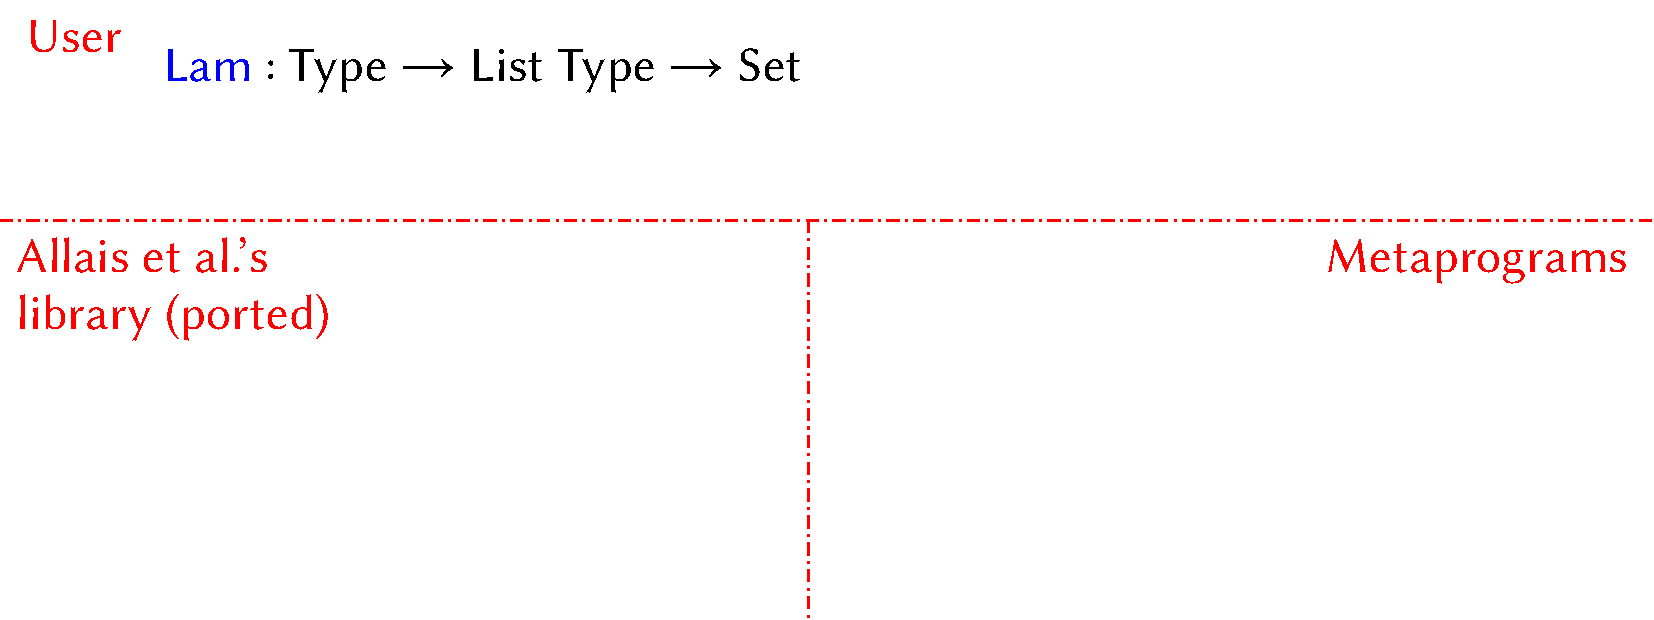
\includegraphics[width=\columnwidth]{Diagram1.pdf}
\end{frame}

\note{Let's do a rundown again, but with our actual definitions. We have three worlds here, the user's own world, the syntax-datatype-generic library, and metaprograms. Say the user defines a language called Lam, indexed by the type and context of a term.}

\begin{frame}[fragile]{Flow Chart}
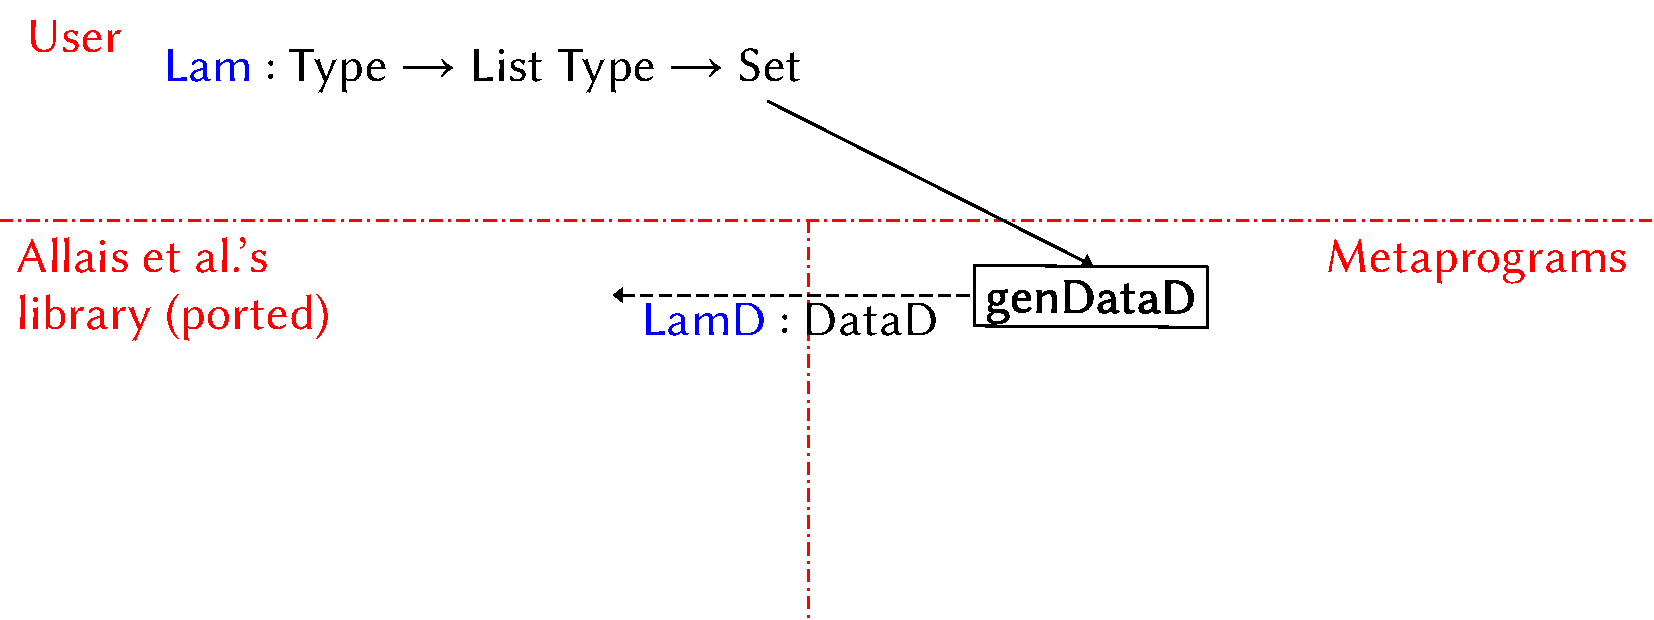
\includegraphics[width=\columnwidth]{Diagram2.pdf}
\end{frame}

\note{They can invoke a metaprogram genDataD, which generates a datatype description of type DataD, we call it LamD.}

\begin{frame}[fragile]{Flow Chart}
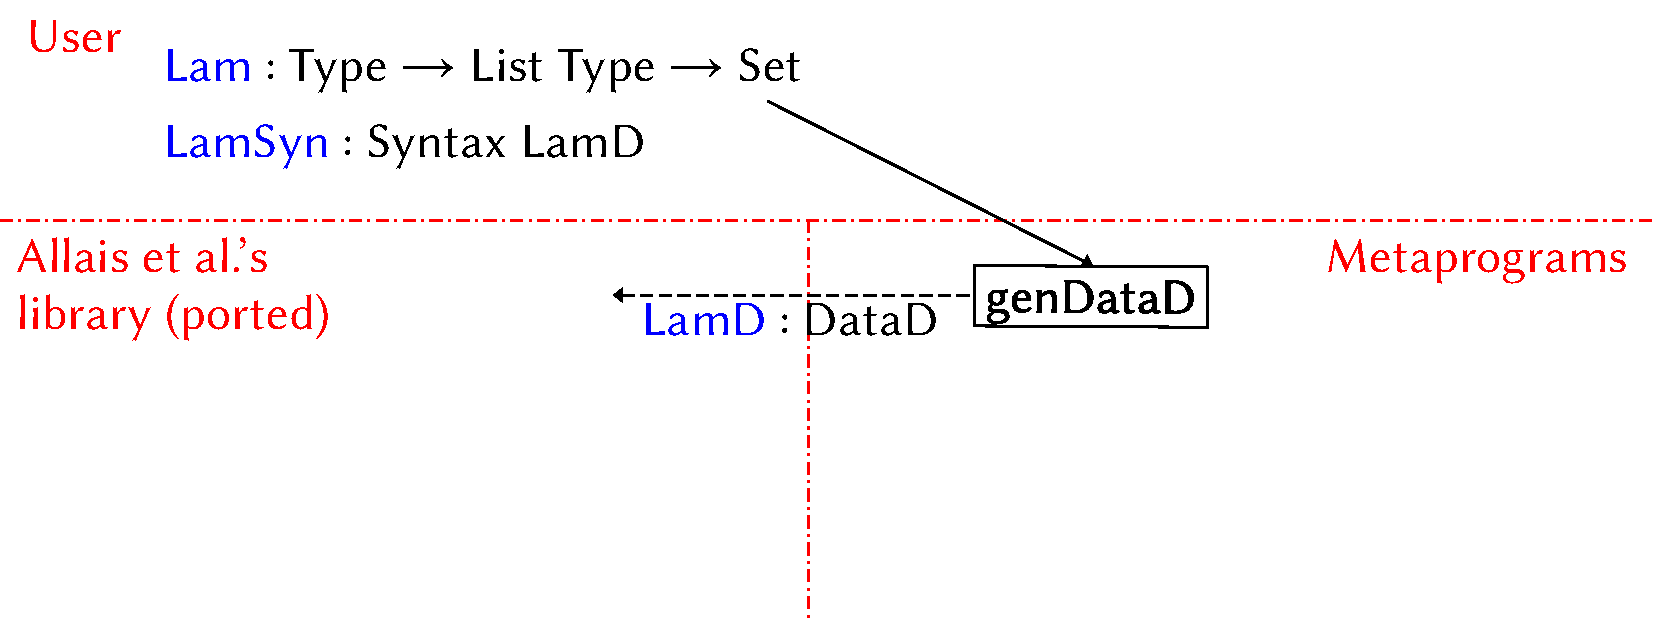
\includegraphics[width=\columnwidth]{Diagram3.pdf}
\end{frame}

\note{Then to use the generic library, the user must provide a proof that the description we just generated is syntax. Here Syntax is the predicate, and we call the proof LamSyn.}

\begin{frame}[fragile]{Flow Chart}
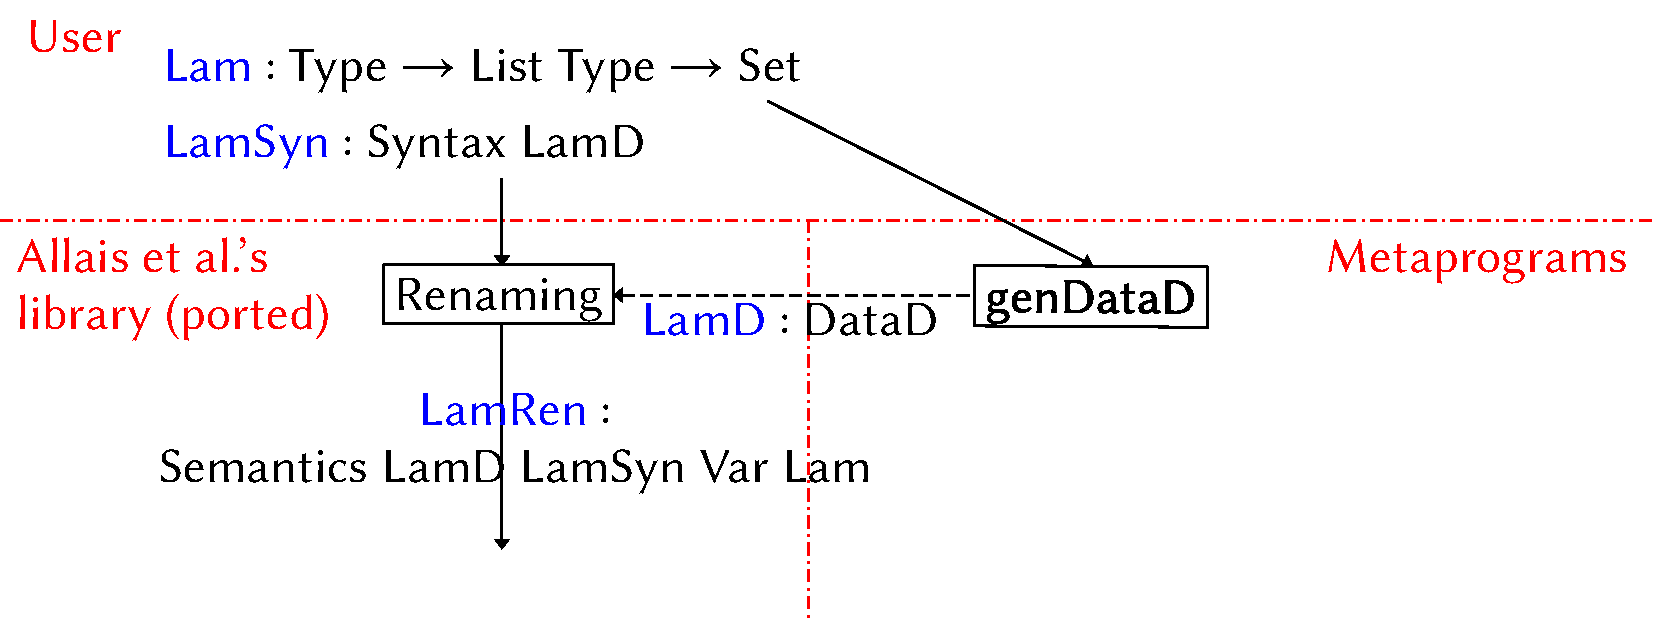
\includegraphics[width=\columnwidth]{Diagram4.pdf}
\end{frame}

\note{Then it's the job for the generic library. Renaming here is a function that generates syntax-generic programs. Syntax-generic programs are represented as Semantics.}

\begin{frame}[fragile]{Flow Chart}
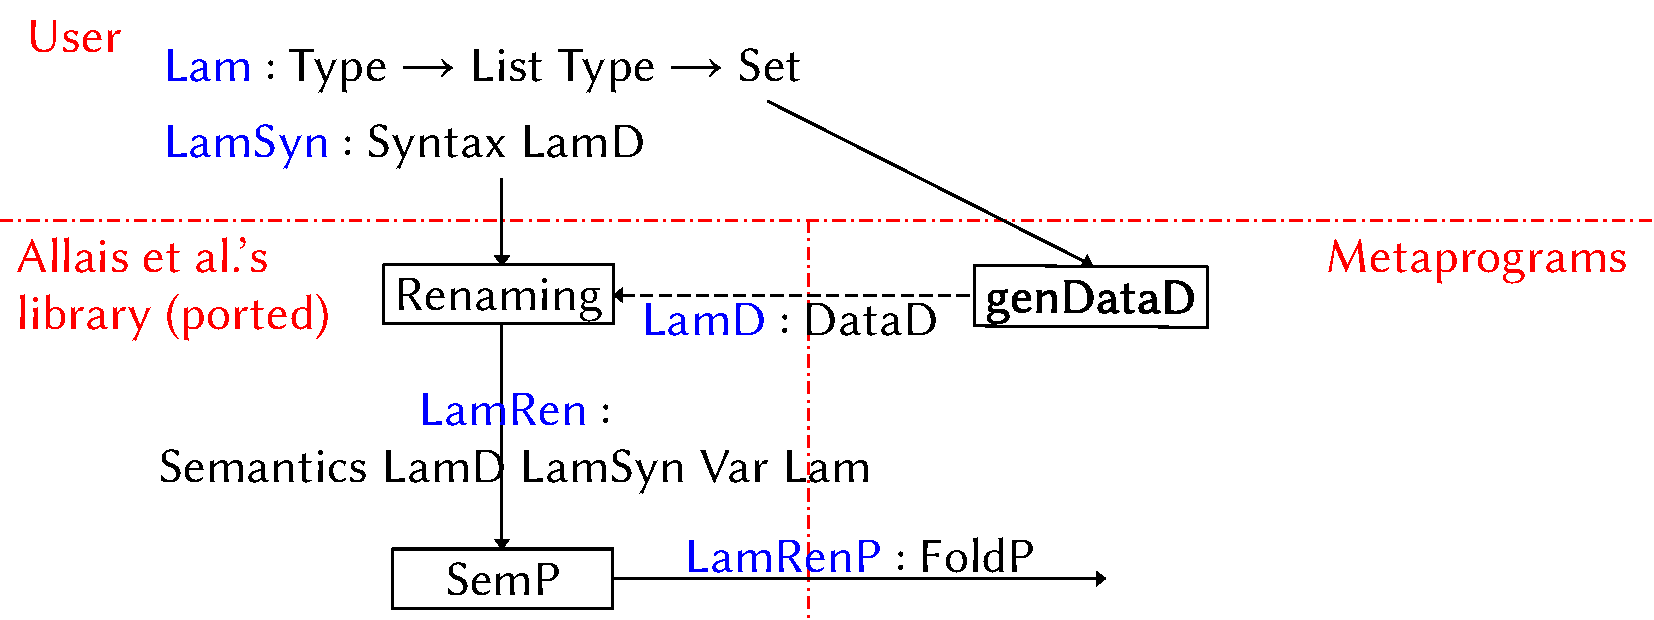
\includegraphics[width=\columnwidth]{Diagram5.pdf}
\end{frame}

\note{But our metaprograms that generates native functions are for datatype-generic programs. so we need another translation in the generic library that is from syntax-generic programs to datatype-generic programs. SemP is this translation and FoldP is the type of datatype-generic fold programs.}

\begin{frame}[fragile]{Flow Chart}
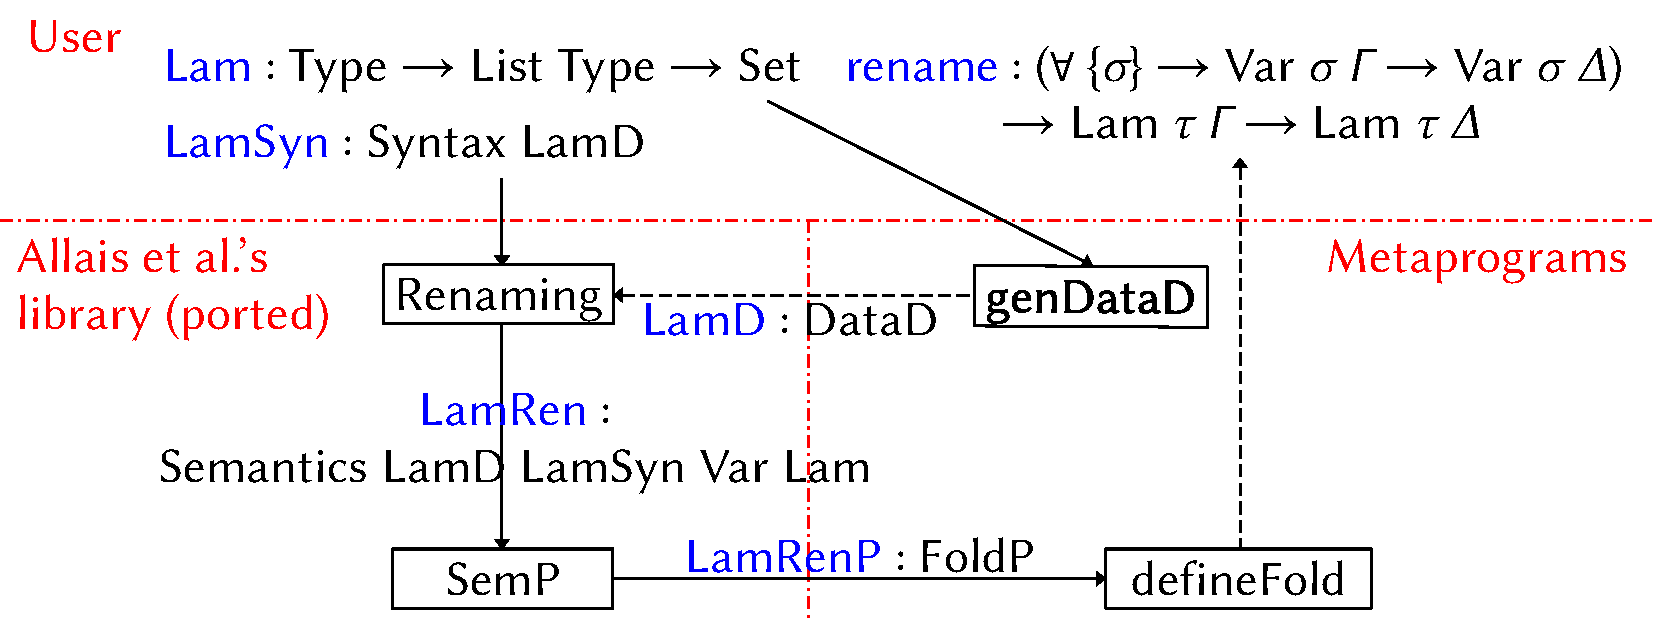
\includegraphics[width=\columnwidth]{Diagram6.pdf}
\end{frame}

\note{Finally, defineFold is a metaprogram that generates actual function definitions. So the user doesn't need to understand the detailed definitions in the generic libary, they can write native datatype and get native function definitions if they know what metaprograms and functions to call.}

\begin{frame}[fragile]{Some of Our Contributions}
In ``Datatype-generic Programming Meets Elaborator Reflection'':
	\begin{itemize}
		\item \mi{DataD}
		\item \mi{FoldP} for folds (and \mi{IndP} for inductions)
		\item metaprogram \mi{genDataD}
		\item metaprogram \mi{defineFold}
	\end{itemize}
\pause
In this work:
	\begin{itemize}
		\item predicate \mi{Syntax} on \mi{DataD} that captures \mi{Desc}.
		\item function \mi{SemP} that generates \mi{FoldP} from \mi{Syntax} proofs.
	\end{itemize}
\end{frame}

\note{The datatype and program descriptions are provided by our other work we mentioned, so are the metaprograms. In this work we provide the Syntax predicate and the translations built arount it.}


\begin{frame}[fragile]{The \mi{Syntax} Predicate}
	\begin{hscode}\SaveRestoreHook
\column{B}{@{}>{\hspre}l<{\hspost}@{}}%
\column{E}{@{}>{\hspre}l<{\hspost}@{}}%
\>[B]{}\Conid{Syntax}\;\mathbin{:}\;\Conid{Set}\;\Varid{ℓ}\;\Varid{→}\;\Conid{DataD}\;\Varid{→}\;\Conid{Setω}{}\<[E]%
\ColumnHook
\end{hscode}\resethooks
\mi{Desc} are captured by \mi{Syntax} as each:
	\pause
	\begin{itemize}
		\item has a variable rule,
		\pause
		\item is not universe polymorphic,
		\pause
		\item has two indices, $I$ and $\mi{List}\ I$, and
		\pause
		\item supports context extensions.
	\end{itemize}
\end{frame}

\note{Unfortunately our time is limited, we can't go into the details of the Syntax predicate.}


\begin{frame}[fragile]{The \mi{Syntax} Predicate}
\begin{columns}[T]
	\begin{column}{0.5\textwidth}
Does \mi{PCF} satisfies \mi{Syntax}?
	\begin{hscode}\SaveRestoreHook
\column{B}{@{}>{\hspre}l<{\hspost}@{}}%
\column{3}{@{}>{\hspre}l<{\hspost}@{}}%
\column{10}{@{}>{\hspre}l<{\hspost}@{}}%
\column{27}{@{}>{\hspre}l<{\hspost}@{}}%
\column{E}{@{}>{\hspre}l<{\hspost}@{}}%
\>[B]{}\mathbf{data}\;\Conid{PCF}\;\mathbin{:}\;\Conid{Ty}\;\Varid{→}\;\Conid{Context}\;\Varid{→}\;\Conid{Set}\;\mathbf{where}{}\<[E]%
\\
\>[B]{}\hsindent{3}{}\<[3]%
\>[3]{}\Varid{‵var}\;{}\<[10]%
\>[10]{}\mathbin{:}\;\Conid{Var}\;\Varid{σ}\;\Conid{Γ}\;\Varid{→}\;\Conid{PCF}\;\Varid{σ}\;\Conid{Γ}{}\<[E]%
\\
\>[B]{}\hsindent{3}{}\<[3]%
\>[3]{}\Varid{‵app}\;{}\<[10]%
\>[10]{}\mathbin{:}\;\Conid{PCF}\;(\Varid{σ}\;\Varid{⇒}\;\Varid{τ})\;\Conid{Γ}\;\Varid{→}\;\Conid{PCF}\;\Varid{σ}\;\Conid{Γ}\;\Varid{→}\;\Conid{PCF}\;\Varid{τ}\;\Conid{Γ}{}\<[E]%
\\
\>[B]{}\hsindent{3}{}\<[3]%
\>[3]{}\Varid{‵lam}\;{}\<[10]%
\>[10]{}\mathbin{:}\;\Conid{PCF}\;\Varid{τ}\;(\Varid{σ}\;\Varid{∷}\;\Conid{Γ})\;{}\<[27]%
\>[27]{}\Varid{→}\;\Conid{PCF}\;(\Varid{σ}\;\Varid{⇒}\;\Varid{τ})\;\Conid{Γ}{}\<[E]%
\\
\>[B]{}\hsindent{3}{}\<[3]%
\>[3]{}\Varid{‵zero}\;{}\<[10]%
\>[10]{}\mathbin{:}\;\Conid{PCF}\;\Varid{‵ℕ}\;\Conid{Γ}{}\<[E]%
\\
\>[B]{}\hsindent{3}{}\<[3]%
\>[3]{}\Varid{‵suc\char95 }\;{}\<[10]%
\>[10]{}\mathbin{:}\;\Conid{PCF}\;\Varid{‵ℕ}\;\Conid{Γ}\;\Varid{→}\;\Conid{PCF}\;\Varid{‵ℕ}\;\Conid{Γ}{}\<[E]%
\ColumnHook
\end{hscode}\resethooks
	\end{column}
	\pause
	\begin{column}{0.5\textwidth}
	Proof of PCF being Syntax:
		\begin{hscode}\SaveRestoreHook
\column{B}{@{}>{\hspre}l<{\hspost}@{}}%
\column{9}{@{}>{\hspre}l<{\hspost}@{}}%
\column{E}{@{}>{\hspre}l<{\hspost}@{}}%
\>[B]{}\Conid{SyntaxPCF}\;\mathbin{:}\;\Conid{Syntax}\;\Conid{Ty}\;(\Varid{genDataD}\;\Conid{PCF}){}\<[E]%
\\
\>[B]{}\Conid{SyntaxPCF}\;\mathrel{=}\;\anonymous \;{}\<[E]%
\\
\>[B]{}\hsindent{9}{}\<[9]%
\>[9]{}\Varid{,}\;\Varid{refl}\;{}\<[E]%
\\
\>[B]{}\hsindent{9}{}\<[9]%
\>[9]{}\Varid{,}\;(\Varid{refl}\;\Varid{,refl})\;{}\<[E]%
\\
\>[B]{}\hsindent{9}{}\<[9]%
\>[9]{}\Varid{,}\;\anonymous \;{}\<[E]%
\\
\>[B]{}\hsindent{9}{}\<[9]%
\>[9]{}\Varid{,}\;\Varid{refl}\;{}\<[E]%
\\
\>[B]{}\hsindent{9}{}\<[9]%
\>[9]{}\Varid{,}\;\Varid{refl}\;{}\<[E]%
\\
\>[B]{}\hsindent{9}{}\<[9]%
\>[9]{}\Varid{,}\;(\anonymous \;\Varid{,}\;\anonymous \;\Varid{,}\;\anonymous \;\Varid{,}\;\Varid{refl}\;\Varid{,}\;(\Varid{λ}\;\anonymous \;\Varid{→}\;\Varid{refl}))\;{}\<[E]%
\\
\>[B]{}\hsindent{9}{}\<[9]%
\>[9]{}\Varid{,}\;(\anonymous \;\Varid{,}\;\anonymous \;\Varid{,}\;\anonymous \;\Varid{,}\;\Varid{refl}\;\Varid{,}\;(\Varid{λ}\;\anonymous \;\Varid{→}\;\Varid{refl}))\;{}\<[E]%
\\
\>[B]{}\hsindent{9}{}\<[9]%
\>[9]{}\Varid{,}\;(\anonymous \;\Varid{,}\;\anonymous \;\Varid{,}\;\anonymous \;\Varid{,}\;\Varid{refl}\;\Varid{,}\;(\Varid{λ}\;\anonymous \;\Varid{→}\;\Varid{refl}))\;{}\<[E]%
\\
\>[B]{}\hsindent{9}{}\<[9]%
\>[9]{}\Varid{,}\;(\anonymous \;\Varid{,}\;\anonymous \;\Varid{,}\;\anonymous \;\Varid{,}\;\Varid{refl}\;\Varid{,}\;(\Varid{λ}\;\anonymous \;\Varid{→}\;\Varid{refl}))\;{}\<[E]%
\\
\>[B]{}\hsindent{9}{}\<[9]%
\>[9]{}\Varid{,}\;\Varid{tt}{}\<[E]%
\ColumnHook
\end{hscode}\resethooks
	\end{column}
\end{columns}
\end{frame}

\note{We were worried that the Syntax proof might be too complicated, because if it's too complicated it would not save any efforts and nobody would want to use it. Fortunately in this case it's pretty straightforward. Suppose we define a language PCF, which has five constructors. For this PCF datatype to be a syntax, a lot of things has to be considered, like the datatype's universe level, numbers of parameters and indices, and constraints on each field of each constructor. In this case the parameters must be empty and there must be exactly two indices, a type and a list of type. It turns out most of these are equality proofs, and if the datatype truely is a syntax, these can be proved by simply using the refl constructor. Proofs of any datatypes being syntaxes look pretty much the same, so it is possible to write yet another metaprogram for generating such proofs. Which is a future work we haven't done yet.}

% \begin{frame}[fragile]{Translation from Semantics to natural looking functions}
% \end{frame}

\section{Discussion}

\begin{frame}[fragile]{Problems with Syntax Universes: Readability}
\begin{columns}[T]
\begin{column}{0.5\textwidth}
	\begin{hscode}\SaveRestoreHook
\column{B}{@{}>{\hspre}l<{\hspost}@{}}%
\column{3}{@{}>{\hspre}l<{\hspost}@{}}%
\column{8}{@{}>{\hspre}l<{\hspost}@{}}%
\column{E}{@{}>{\hspre}l<{\hspost}@{}}%
\>[B]{}\mathbf{data}\;\Varid{\char95 ⊢\char95 }\;\mathbin{:}\;\Conid{Context}\;\Varid{→}\;\Conid{Ty}\;\Varid{→}\;\Conid{Set}\;\mathbf{where}{}\<[E]%
\\
\>[B]{}\hsindent{3}{}\<[3]%
\>[3]{}\Varid{‵\char95 }\;{}\<[8]%
\>[8]{}\mathbin{:}\;\Conid{Γ}\;\Varid{∋}\;\Conid{A}\;\Varid{→}\;\Conid{Γ}\;\Varid{⊢}\;\Conid{A}{}\<[E]%
\\
\>[B]{}\hsindent{3}{}\<[3]%
\>[3]{}\Varid{ƛ\char95 }\;{}\<[8]%
\>[8]{}\mathbin{:}\;\Conid{Γ}\;\Varid{,}\;\Conid{A}\;\Varid{⊢}\;\Conid{B}\;\Varid{→}\;\Conid{Γ}\;\Varid{⊢}\;\Conid{A}\;\Varid{⇒}\;\Conid{B}{}\<[E]%
\\
\>[B]{}\hsindent{3}{}\<[3]%
\>[3]{}\Varid{\char95 ·\char95 }\;{}\<[8]%
\>[8]{}\mathbin{:}\;\Conid{Γ}\;\Varid{⊢}\;\Conid{A}\;\Varid{⇒}\;\Conid{B}\;\Varid{→}\;\Conid{Γ}\;\Varid{⊢}\;\Conid{A}\;\Varid{→}\;\Conid{Γ}\;\Varid{⊢}\;\Conid{B}{}\<[E]%
\ColumnHook
\end{hscode}\resethooks
\end{column}
\begin{column}{0.5\textwidth}
	\begin{hscode}\SaveRestoreHook
\column{B}{@{}>{\hspre}l<{\hspost}@{}}%
\column{3}{@{}>{\hspre}l<{\hspost}@{}}%
\column{5}{@{}>{\hspre}l<{\hspost}@{}}%
\column{9}{@{}>{\hspre}l<{\hspost}@{}}%
\column{E}{@{}>{\hspre}l<{\hspost}@{}}%
\>[B]{}\Conid{STLCD}\;\mathbin{:}\;\Conid{Desc}\;\Conid{Ty}{}\<[E]%
\\
\>[B]{}\Conid{STLCD}\;\mathrel{=}\;\Varid{‵σ}\;\Varid{‵STLC}\;\Varid{λ}\;\mathbf{where}{}\<[E]%
\\
\>[B]{}\hsindent{3}{}\<[3]%
\>[3]{}(\Conid{App}\;{}\<[9]%
\>[9]{}\Varid{i}\;\Varid{j})\;\Varid{→}\;{}\<[E]%
\\
\>[3]{}\hsindent{2}{}\<[5]%
\>[5]{}\Varid{‵X}\;\Varid{[]}\;(\Varid{i}\;\Varid{⇒}\;\Varid{j})\;(\Varid{‵X}\;\Varid{[]}\;\Varid{i}\;(\Varid{▪}\;\Varid{j})){}\<[E]%
\\
\>[B]{}\hsindent{3}{}\<[3]%
\>[3]{}(\Conid{Lam}\;{}\<[9]%
\>[9]{}\Varid{i}\;\Varid{j})\;\Varid{→}\;{}\<[E]%
\\
\>[3]{}\hsindent{2}{}\<[5]%
\>[5]{}\Varid{‵X}\;(\Varid{i}\;\Varid{∷}\;\Varid{[]})\;\Varid{j}\;(\Varid{▪}\;(\Varid{i}\;\Varid{⇒}\;\Varid{j})){}\<[E]%
\\[\blanklineskip]%
\>[B]{}\Conid{STLC'}\;\mathrel{=}\;\Conid{Tm}\;\Conid{STLCD}{}\<[E]%
\ColumnHook
\end{hscode}\resethooks
\end{column}
\end{columns}
\end{frame}

\note{We quickly summerize what we think are the reasons these libraries are not widely adopted. First of all is readability. One good thing about of intrinsic typing is that types of constructors closely resemble typing rules, and typing rules are less obvious for syntaxes defined in generic universes.}

\begin{frame}[fragile]{Problems with Syntax Universes: Burden on Programmers}
	\begin{hscode}\SaveRestoreHook
\column{B}{@{}>{\hspre}l<{\hspost}@{}}%
\column{9}{@{}>{\hspre}l<{\hspost}@{}}%
\column{13}{@{}>{\hspre}l<{\hspost}@{}}%
\column{E}{@{}>{\hspre}l<{\hspost}@{}}%
\>[B]{}\mathbf{data}\;\Conid{Desc}\;(\Conid{I}\;\mathbin{:}\;\Conid{Set})\;\mathbin{:}\;\Conid{Set₁}\;\mathbf{where}{}\<[E]%
\\
\>[B]{}\hsindent{9}{}\<[9]%
\>[9]{}\Varid{‵σ}\;{}\<[13]%
\>[13]{}\mathbin{:}\;(\Conid{A}\;\mathbin{:}\;\Conid{Set})\;\Varid{→}\;(\Conid{A}\;\Varid{→}\;\Conid{Desc}\;\Conid{I})\;\Varid{→}\;\Conid{Desc}\;\Conid{I}{}\<[E]%
\\
\>[B]{}\hsindent{9}{}\<[9]%
\>[9]{}\Varid{‵X}\;{}\<[13]%
\>[13]{}\mathbin{:}\;\Conid{List}\;\Conid{I}\;\Varid{→}\;\Conid{I}\;\Varid{→}\;\Conid{Desc}\;\Conid{I}\;\Varid{→}\;\Conid{Desc}\;\Conid{I}{}\<[E]%
\\
\>[B]{}\hsindent{9}{}\<[9]%
\>[9]{}\Varid{‵▪}\;{}\<[13]%
\>[13]{}\mathbin{:}\;\Conid{I}\;\Varid{→}\;\Conid{Desc}\;\Conid{I}{}\<[E]%
\ColumnHook
\end{hscode}\resethooks
\end{frame}

\note{Secondly, to utilize such generic libraries, programmers are required to understand the generic universe instead of just defining syntaxes the way they want. }

\begin{frame}[fragile]{Problems with Syntax Universes: Interoperability}
	\begin{hscode}\SaveRestoreHook
\column{B}{@{}>{\hspre}l<{\hspost}@{}}%
\column{E}{@{}>{\hspre}l<{\hspost}@{}}%
\>[B]{}\Conid{STLCD}\;\mathbin{:}\;\Conid{Desc}\;\Conid{Ty}{}\<[E]%
\\
\>[B]{}\Conid{STLCD}\;\mathrel{=}\;\Varid{...}{}\<[E]%
\\[\blanklineskip]%
\>[B]{}\Conid{STLCD'}\;\mathbin{:}\;\Conid{Desc'}\;\Varid{???}{}\<[E]%
\\
\>[B]{}\Conid{STLCD'}\;\mathrel{=}\;\Varid{???}{}\<[E]%
\ColumnHook
\end{hscode}\resethooks
\end{frame}

\note{And they need to learn a new generic representation everytime they want some features that only exist in another generic library, the syntax they are working on must be redefined. This leads us to te third problem, interoperability. It would be hard to use two or more generic libraries at once.}

\begin{frame}[fragile]{Towards Datatype-generic Libraries for Syntaxes?}
		% \item Expressiveness is limited by Agda datatypes as well as the generic universe, a \mi{Syntax} predicate must be defined.
		% \pause
		% \item Even if we can define \mi{Syntax}, the proof could be more complicated, even require programmers to understand the generic universe.
		% \pause
		% \item Obstacles of using multiple generic libraries at once.
		% \pause
		% \item Are folds and inductions enough?
		\begin{itemize}
			\item Do we really need syntax-generic libraries?
		\end{itemize}
\end{frame}

\note{What about our approach? our work has a lot to be done. Since we are running out of time, I would like to address one issue that's probably the elephant in the room. What if people actually don't want syntax-generic operations at all? Maybe they only define a language once in a while, and it's not worth the time looking up what libraries they can use. Or, since researchers define languages with new features all the time, maybe it's common for them to come up something no generic universes can cover. Our framework could still be help in that case, maybe our metaprograms can analyse the constructors in a datatype and determine which of them fit in a universe, and generate functions that are partially defined, then leave the uncertain parts to the programmer. So what do you think about it? Please share with us your conerns or what you think this framework can be going. Thank you all for listening.}

\end{document}

